\documentclass[twoside]{book}

% Packages required by doxygen
\usepackage{calc}
\usepackage{doxygen}
\usepackage{graphicx}
\usepackage[utf8]{inputenc}
\usepackage{makeidx}
\usepackage{multicol}
\usepackage{multirow}
\usepackage{textcomp}
\usepackage[table]{xcolor}

% Font selection
\usepackage[T1]{fontenc}
\usepackage{mathptmx}
\usepackage[scaled=.90]{helvet}
\usepackage{courier}
\usepackage{amssymb}
\usepackage{sectsty}
\renewcommand{\familydefault}{\sfdefault}
\allsectionsfont{%
  \fontseries{bc}\selectfont%
  \color{darkgray}%
}
\renewcommand{\DoxyLabelFont}{%
  \fontseries{bc}\selectfont%
  \color{darkgray}%
}

% Page & text layout
\usepackage{geometry}
\geometry{%
  a4paper,%
  top=2.5cm,%
  bottom=2.5cm,%
  left=2.5cm,%
  right=2.5cm%
}
\tolerance=750
\hfuzz=15pt
\hbadness=750
\setlength{\emergencystretch}{15pt}
\setlength{\parindent}{0cm}
\setlength{\parskip}{0.2cm}
\makeatletter
\renewcommand{\paragraph}{%
  \@startsection{paragraph}{4}{0ex}{-1.0ex}{1.0ex}{%
    \normalfont\normalsize\bfseries\SS@parafont%
  }%
}
\renewcommand{\subparagraph}{%
  \@startsection{subparagraph}{5}{0ex}{-1.0ex}{1.0ex}{%
    \normalfont\normalsize\bfseries\SS@subparafont%
  }%
}
\makeatother

% Headers & footers
\usepackage{fancyhdr}
\pagestyle{fancyplain}
\fancyhead[LE]{\fancyplain{}{\bfseries\thepage}}
\fancyhead[CE]{\fancyplain{}{}}
\fancyhead[RE]{\fancyplain{}{\bfseries\leftmark}}
\fancyhead[LO]{\fancyplain{}{\bfseries\rightmark}}
\fancyhead[CO]{\fancyplain{}{}}
\fancyhead[RO]{\fancyplain{}{\bfseries\thepage}}
\fancyfoot[LE]{\fancyplain{}{}}
\fancyfoot[CE]{\fancyplain{}{}}
\fancyfoot[RE]{\fancyplain{}{\bfseries\scriptsize Generated on Fri Aug 28 2015 15\-:59\-:43 for Cloth\-Sim by Doxygen }}
\fancyfoot[LO]{\fancyplain{}{\bfseries\scriptsize Generated on Fri Aug 28 2015 15\-:59\-:43 for Cloth\-Sim by Doxygen }}
\fancyfoot[CO]{\fancyplain{}{}}
\fancyfoot[RO]{\fancyplain{}{}}
\renewcommand{\footrulewidth}{0.4pt}
\renewcommand{\chaptermark}[1]{%
  \markboth{#1}{}%
}
\renewcommand{\sectionmark}[1]{%
  \markright{\thesection\ #1}%
}

% Indices & bibliography
\usepackage{natbib}
\usepackage[titles]{tocloft}
\setcounter{tocdepth}{3}
\setcounter{secnumdepth}{5}
\makeindex

% Hyperlinks (required, but should be loaded last)
\usepackage{ifpdf}
\ifpdf
  \usepackage[pdftex,pagebackref=true]{hyperref}
\else
  \usepackage[ps2pdf,pagebackref=true]{hyperref}
\fi
\hypersetup{%
  colorlinks=true,%
  linkcolor=blue,%
  citecolor=blue,%
  unicode%
}

% Custom commands
\newcommand{\clearemptydoublepage}{%
  \newpage{\pagestyle{empty}\cleardoublepage}%
}


%===== C O N T E N T S =====

\begin{document}

% Titlepage & ToC
\hypersetup{pageanchor=false}
\pagenumbering{roman}
\begin{titlepage}
\vspace*{7cm}
\begin{center}%
{\Large Cloth\-Sim \\[1ex]\large 1.\-0 }\\
\vspace*{1cm}
{\large Generated by Doxygen 1.8.6}\\
\vspace*{0.5cm}
{\small Fri Aug 28 2015 15:59:43}\\
\end{center}
\end{titlepage}
\clearemptydoublepage
\tableofcontents
\clearemptydoublepage
\pagenumbering{arabic}
\hypersetup{pageanchor=true}

%--- Begin generated contents ---
\chapter{Install instrustions}
\label{md__r_e_a_d_m_e}
\hypertarget{md__r_e_a_d_m_e}{}
A fluid simulation for my advanced graphics software development techniques unit. This is an S\-P\-H Fluid simulation that uses dynamic parallelism and fancy shading techniques.

Instalation and running\-:

For this simulation to run your G\-P\-U will need the to have compatibility with cuda and dynamic Parallelism. This will require an N\-Vidia chip of compute caperbility 3.\-5 or higher! It should work on both mac and linux but I have not tested for mac so don't hold me to this!

Step 1\-: You will need to tweak your gencode caperbility in the .pro file to your hardware configuration. Step 2\-: (optional) Depending on what version on cuda you are running you may have to change the path to your cuda library in the .pro aswell. Im running 6.\-5 so if you are the same you should be fine. Step 3\-: In the A\-G\-S\-D\-T\-Fluid\-Sim directory run, \begin{DoxyVerb}qmake
make clean
make
\end{DoxyVerb}


step 4\-: You should now have a working executable. Please contact me if you cant get it working.

Documentation and Report\-:

The documation and report of this project are in the form of a doxygen file. To access this you can either run the program and open it with the \char`\"{}\-Open Documenation\char`\"{} button or open index.\-html which you will find in doc/html/

Enjoy!

Dec 
\chapter{Todo List}
\label{todo}
\hypertarget{todo}{}

\begin{DoxyRefList}
\item[\label{todo__todo000001}%
\hypertarget{todo__todo000001}{}%
File \hyperlink{_camera_8h}{Camera.h} ]Rewrite Tobies shitty \hyperlink{class_camera}{Camera} class. Its not even commented!! F\-F\-S T\-O\-B\-Y! U\-S\-E\-L\-E\-S\-S!!!  
\item[\label{todo__todo000002}%
\hypertarget{todo__todo000002}{}%
File \hyperlink{_text_8h}{Text.h} ]support unicode A\-S\-C\-I\-I is so 1980's ;-\/0 This class will generate billboard textures and Vertex\-Array\-Objects for each of the font glyphs, this means we need a valid Open\-G\-L context before using this class, therefore it should be constructed in initalize\-G\-L or after. Note for efficiency once the font has been created we can only change the colour, if you need different sizes / emphasis you will need to create a new \hyperlink{class_text}{Text} object with the desired size / emphasis. This is accelerated as much as possible but text rendering will sometimes be slow as we bind a new texture for each char being drawn for more details look at the blog post here \href{http://jonmacey.blogspot.com/2011/10/text-rendering-using-opengl-32.html}{\tt http\-://jonmacey.\-blogspot.\-com/2011/10/text-\/rendering-\/using-\/opengl-\/32.\-html} 
\end{DoxyRefList}
\chapter{Hierarchical Index}
\section{Class Hierarchy}
This inheritance list is sorted roughly, but not completely, alphabetically\-:\begin{DoxyCompactList}
\item \contentsline{section}{Abstract\-Open\-Gl\-Object}{\pageref{class_abstract_open_gl_object}}{}
\begin{DoxyCompactList}
\item \contentsline{section}{Frame\-Buffer}{\pageref{class_frame_buffer}}{}
\item \contentsline{section}{G\-L\-Texture}{\pageref{class_g_l_texture}}{}
\item \contentsline{section}{Render\-Buffer}{\pageref{class_render_buffer}}{}
\end{DoxyCompactList}
\item \contentsline{section}{Abstract\-Render\-Target}{\pageref{class_abstract_render_target}}{}
\item \contentsline{section}{Camera}{\pageref{class_camera}}{}
\item \contentsline{section}{Text\-:\-:Font\-Char}{\pageref{struct_text_1_1_font_char}}{}
\item \contentsline{section}{G\-L\-Texture\-Lib}{\pageref{class_g_l_texture_lib}}{}
\item Q\-G\-L\-Widget\begin{DoxyCompactList}
\item \contentsline{section}{Open\-G\-L\-Widget}{\pageref{class_open_g_l_widget}}{}
\end{DoxyCompactList}
\item Q\-Main\-Window\begin{DoxyCompactList}
\item \contentsline{section}{Main\-Window}{\pageref{class_main_window}}{}
\end{DoxyCompactList}
\item \contentsline{section}{qt\-\_\-meta\-\_\-stringdata\-\_\-\-Fluid\-Prop\-Dock\-Widget\-\_\-t}{\pageref{structqt__meta__stringdata___fluid_prop_dock_widget__t}}{}
\item \contentsline{section}{qt\-\_\-meta\-\_\-stringdata\-\_\-\-Main\-Window\-\_\-t}{\pageref{structqt__meta__stringdata___main_window__t}}{}
\item \contentsline{section}{qt\-\_\-meta\-\_\-stringdata\-\_\-\-Open\-G\-L\-Widget\-\_\-t}{\pageref{structqt__meta__stringdata___open_g_l_widget__t}}{}
\item \contentsline{section}{Render\-Target\-Lib}{\pageref{class_render_target_lib}}{}
\item \contentsline{section}{Shader}{\pageref{class_shader}}{}
\item \contentsline{section}{Shader\-Program}{\pageref{class_shader_program}}{}
\item \contentsline{section}{shader\-Utils}{\pageref{classshader_utils}}{}
\item \contentsline{section}{Text}{\pageref{class_text}}{}
\item \contentsline{section}{Ui\-\_\-\-Main\-Window}{\pageref{class_ui___main_window}}{}
\begin{DoxyCompactList}
\item \contentsline{section}{Ui\-:\-:Main\-Window}{\pageref{class_ui_1_1_main_window}}{}
\end{DoxyCompactList}
\end{DoxyCompactList}

\chapter{Class Index}
\section{Class List}
Here are the classes, structs, unions and interfaces with brief descriptions\-:\begin{DoxyCompactList}
\item\contentsline{section}{\hyperlink{class_abstract_open_gl_object}{Abstract\-Open\-Gl\-Object} }{\pageref{class_abstract_open_gl_object}}{}
\item\contentsline{section}{\hyperlink{class_abstract_render_target}{Abstract\-Render\-Target} \\*Abstract base class for Open\-G\-L Objects }{\pageref{class_abstract_render_target}}{}
\item\contentsline{section}{\hyperlink{class_camera}{Camera} }{\pageref{class_camera}}{}
\item\contentsline{section}{\hyperlink{struct_text_1_1_font_char}{Text\-::\-Font\-Char} \\*Structure to hold the font char texture id and the vao. The vao for each font will be a different size need to investigate is a scale would be quicker / more efficient than storing multiple billboards (some will be the same size) }{\pageref{struct_text_1_1_font_char}}{}
\item\contentsline{section}{\hyperlink{class_frame_buffer}{Frame\-Buffer} \\*Class for creating frame buffers }{\pageref{class_frame_buffer}}{}
\item\contentsline{section}{\hyperlink{class_g_l_texture}{G\-L\-Texture} }{\pageref{class_g_l_texture}}{}
\item\contentsline{section}{\hyperlink{class_g_l_texture_lib}{G\-L\-Texture\-Lib} \\*Simple class for loading in and managing Open\-G\-L textures }{\pageref{class_g_l_texture_lib}}{}
\item\contentsline{section}{\hyperlink{class_ui_1_1_main_window}{Ui\-::\-Main\-Window} }{\pageref{class_ui_1_1_main_window}}{}
\item\contentsline{section}{\hyperlink{class_main_window}{Main\-Window} }{\pageref{class_main_window}}{}
\item\contentsline{section}{\hyperlink{class_open_g_l_widget}{Open\-G\-L\-Widget} \\*Basic Qt widget that holds a Open\-G\-L context }{\pageref{class_open_g_l_widget}}{}
\item\contentsline{section}{\hyperlink{structqt__meta__stringdata___fluid_prop_dock_widget__t}{qt\-\_\-meta\-\_\-stringdata\-\_\-\-Fluid\-Prop\-Dock\-Widget\-\_\-t} }{\pageref{structqt__meta__stringdata___fluid_prop_dock_widget__t}}{}
\item\contentsline{section}{\hyperlink{structqt__meta__stringdata___main_window__t}{qt\-\_\-meta\-\_\-stringdata\-\_\-\-Main\-Window\-\_\-t} }{\pageref{structqt__meta__stringdata___main_window__t}}{}
\item\contentsline{section}{\hyperlink{structqt__meta__stringdata___open_g_l_widget__t}{qt\-\_\-meta\-\_\-stringdata\-\_\-\-Open\-G\-L\-Widget\-\_\-t} }{\pageref{structqt__meta__stringdata___open_g_l_widget__t}}{}
\item\contentsline{section}{\hyperlink{class_render_buffer}{Render\-Buffer} \\*Class for creating render buffers }{\pageref{class_render_buffer}}{}
\item\contentsline{section}{\hyperlink{class_render_target_lib}{Render\-Target\-Lib} \\*Singleton class for creating and storing render targets in a library }{\pageref{class_render_target_lib}}{}
\item\contentsline{section}{\hyperlink{class_shader}{Shader} }{\pageref{class_shader}}{}
\item\contentsline{section}{\hyperlink{class_shader_program}{Shader\-Program} }{\pageref{class_shader_program}}{}
\item\contentsline{section}{\hyperlink{classshader_utils}{shader\-Utils} }{\pageref{classshader_utils}}{}
\item\contentsline{section}{\hyperlink{class_text}{Text} }{\pageref{class_text}}{}
\item\contentsline{section}{\hyperlink{class_ui___main_window}{Ui\-\_\-\-Main\-Window} }{\pageref{class_ui___main_window}}{}
\end{DoxyCompactList}

\chapter{File Index}
\section{File List}
Here is a list of all documented files with brief descriptions\-:\begin{DoxyCompactList}
\item\contentsline{section}{/home/dexternation/\-A\-G\-S\-D\-T\-Fluid\-Sim/{\bfseries ui\-\_\-mainwindow.\-h} }{\pageref{ui__mainwindow_8h}}{}
\item\contentsline{section}{/home/dexternation/\-A\-G\-S\-D\-T\-Fluid\-Sim/cuda\-Src/\hyperlink{_cuda_s_p_h_kernals_8cu}{Cuda\-S\-P\-H\-Kernals.\-cu} }{\pageref{_cuda_s_p_h_kernals_8cu}}{}
\item\contentsline{section}{/home/dexternation/\-A\-G\-S\-D\-T\-Fluid\-Sim/include/{\bfseries Abstract\-Open\-G\-L\-Object.\-h} }{\pageref{_abstract_open_g_l_object_8h}}{}
\item\contentsline{section}{/home/dexternation/\-A\-G\-S\-D\-T\-Fluid\-Sim/include/\hyperlink{_cuda_s_p_h_kernals_8h}{Cuda\-S\-P\-H\-Kernals.\-h} \\*Used for prototyping our our functions used for our S\-P\-H simulation calculations }{\pageref{_cuda_s_p_h_kernals_8h}}{}
\item\contentsline{section}{/home/dexternation/\-A\-G\-S\-D\-T\-Fluid\-Sim/include/{\bfseries Fluid\-Prop\-Dock\-Widget.\-h} }{\pageref{_fluid_prop_dock_widget_8h}}{}
\item\contentsline{section}{/home/dexternation/\-A\-G\-S\-D\-T\-Fluid\-Sim/include/\hyperlink{_fluid_shader_8h}{Fluid\-Shader.\-h} }{\pageref{_fluid_shader_8h}}{}
\item\contentsline{section}{/home/dexternation/\-A\-G\-S\-D\-T\-Fluid\-Sim/include/\hyperlink{_frame_buffer_8h}{Frame\-Buffer.\-h} }{\pageref{_frame_buffer_8h}}{}
\item\contentsline{section}{/home/dexternation/\-A\-G\-S\-D\-T\-Fluid\-Sim/include/\hyperlink{_g_l_texture_8h}{G\-L\-Texture.\-h} }{\pageref{_g_l_texture_8h}}{}
\item\contentsline{section}{/home/dexternation/\-A\-G\-S\-D\-T\-Fluid\-Sim/include/\hyperlink{_g_l_texture_lib_8h}{G\-L\-Texture\-Lib.\-h} }{\pageref{_g_l_texture_lib_8h}}{}
\item\contentsline{section}{/home/dexternation/\-A\-G\-S\-D\-T\-Fluid\-Sim/include/{\bfseries helper\-\_\-math.\-h} }{\pageref{helper__math_8h}}{}
\item\contentsline{section}{/home/dexternation/\-A\-G\-S\-D\-T\-Fluid\-Sim/include/{\bfseries mainwindow.\-h} }{\pageref{mainwindow_8h}}{}
\item\contentsline{section}{/home/dexternation/\-A\-G\-S\-D\-T\-Fluid\-Sim/include/\hyperlink{_open_g_l_widget_8h}{Open\-G\-L\-Widget.\-h} }{\pageref{_open_g_l_widget_8h}}{}
\item\contentsline{section}{/home/dexternation/\-A\-G\-S\-D\-T\-Fluid\-Sim/include/\hyperlink{_render_buffer_8h}{Render\-Buffer.\-h} }{\pageref{_render_buffer_8h}}{}
\item\contentsline{section}{/home/dexternation/\-A\-G\-S\-D\-T\-Fluid\-Sim/include/\hyperlink{_render_target_lib_8h}{Render\-Target\-Lib.\-h} }{\pageref{_render_target_lib_8h}}{}
\item\contentsline{section}{/home/dexternation/\-A\-G\-S\-D\-T\-Fluid\-Sim/include/\hyperlink{_s_p_h_engine_8h}{S\-P\-H\-Engine.\-h} }{\pageref{_s_p_h_engine_8h}}{}
\item\contentsline{section}{/home/dexternation/\-A\-G\-S\-D\-T\-Fluid\-Sim/include/{\bfseries ui\-\_\-mainwindow.\-h} }{\pageref{include_2ui__mainwindow_8h}}{}
\item\contentsline{section}{/home/dexternation/\-A\-G\-S\-D\-T\-Fluid\-Sim/shaders/\hyperlink{bilateral_filter_frag_8glsl}{bilateral\-Filter\-Frag.\-glsl} }{\pageref{bilateral_filter_frag_8glsl}}{}
\item\contentsline{section}{/home/dexternation/\-A\-G\-S\-D\-T\-Fluid\-Sim/shaders/\hyperlink{bilateral_filter_vert_8glsl}{bilateral\-Filter\-Vert.\-glsl} }{\pageref{bilateral_filter_vert_8glsl}}{}
\item\contentsline{section}{/home/dexternation/\-A\-G\-S\-D\-T\-Fluid\-Sim/shaders/\hyperlink{cuboid_geom_8glsl}{cuboid\-Geom.\-glsl} }{\pageref{cuboid_geom_8glsl}}{}
\item\contentsline{section}{/home/dexternation/\-A\-G\-S\-D\-T\-Fluid\-Sim/shaders/\hyperlink{cuboid_vert_8glsl}{cuboid\-Vert.\-glsl} }{\pageref{cuboid_vert_8glsl}}{}
\item\contentsline{section}{/home/dexternation/\-A\-G\-S\-D\-T\-Fluid\-Sim/shaders/\hyperlink{fluid_shader_frag_8glsl}{fluid\-Shader\-Frag.\-glsl} }{\pageref{fluid_shader_frag_8glsl}}{}
\item\contentsline{section}{/home/dexternation/\-A\-G\-S\-D\-T\-Fluid\-Sim/shaders/\hyperlink{fluid_shader_vert_8glsl}{fluid\-Shader\-Vert.\-glsl} }{\pageref{fluid_shader_vert_8glsl}}{}
\item\contentsline{section}{/home/dexternation/\-A\-G\-S\-D\-T\-Fluid\-Sim/shaders/\hyperlink{particle_depth_frag_8glsl}{particle\-Depth\-Frag.\-glsl} }{\pageref{particle_depth_frag_8glsl}}{}
\item\contentsline{section}{/home/dexternation/\-A\-G\-S\-D\-T\-Fluid\-Sim/shaders/\hyperlink{particle_depth_vert_8glsl}{particle\-Depth\-Vert.\-glsl} }{\pageref{particle_depth_vert_8glsl}}{}
\item\contentsline{section}{/home/dexternation/\-A\-G\-S\-D\-T\-Fluid\-Sim/shaders/\hyperlink{sky_box_frag_8glsl}{sky\-Box\-Frag.\-glsl} }{\pageref{sky_box_frag_8glsl}}{}
\item\contentsline{section}{/home/dexternation/\-A\-G\-S\-D\-T\-Fluid\-Sim/shaders/\hyperlink{sky_box_vert_8glsl}{sky\-Box\-Vert.\-glsl} }{\pageref{sky_box_vert_8glsl}}{}
\item\contentsline{section}{/home/dexternation/\-A\-G\-S\-D\-T\-Fluid\-Sim/shaders/\hyperlink{thickness_frag_8glsl}{thickness\-Frag.\-glsl} }{\pageref{thickness_frag_8glsl}}{}
\item\contentsline{section}{/home/dexternation/\-A\-G\-S\-D\-T\-Fluid\-Sim/shaders/\hyperlink{thickness_vert_8glsl}{thickness\-Vert.\-glsl} }{\pageref{thickness_vert_8glsl}}{}
\end{DoxyCompactList}

\chapter{Class Documentation}
\hypertarget{class_abstract_open_gl_object}{\section{Abstract\-Open\-Gl\-Object Class Reference}
\label{class_abstract_open_gl_object}\index{Abstract\-Open\-Gl\-Object@{Abstract\-Open\-Gl\-Object}}
}


Inheritance diagram for Abstract\-Open\-Gl\-Object\-:


Collaboration diagram for Abstract\-Open\-Gl\-Object\-:
\subsection*{Public Member Functions}
\begin{DoxyCompactItemize}
\item 
\hypertarget{class_abstract_open_gl_object_a96af8fad4e89a9ea75c535748ffa82a5}{\hyperlink{class_abstract_open_gl_object_a96af8fad4e89a9ea75c535748ffa82a5}{Abstract\-Open\-Gl\-Object} ()}\label{class_abstract_open_gl_object_a96af8fad4e89a9ea75c535748ffa82a5}

\begin{DoxyCompactList}\small\item\em default constructor, does nothing \end{DoxyCompactList}\item 
\hypertarget{class_abstract_open_gl_object_ac48ade8b59e497ef45e9238327f93873}{virtual \hyperlink{class_abstract_open_gl_object_ac48ade8b59e497ef45e9238327f93873}{$\sim$\-Abstract\-Open\-Gl\-Object} ()}\label{class_abstract_open_gl_object_ac48ade8b59e497ef45e9238327f93873}

\begin{DoxyCompactList}\small\item\em defalut destructor \end{DoxyCompactList}\item 
\hypertarget{class_abstract_open_gl_object_ad177ced7b2eee2b6d80faa8f5409517b}{virtual void \hyperlink{class_abstract_open_gl_object_ad177ced7b2eee2b6d80faa8f5409517b}{bind} ()}\label{class_abstract_open_gl_object_ad177ced7b2eee2b6d80faa8f5409517b}

\begin{DoxyCompactList}\small\item\em virtual method to bind our open\-G\-L object \end{DoxyCompactList}\item 
\hypertarget{class_abstract_open_gl_object_aa345bb3bc9d0e27521462fd3cfa93a69}{virtual void \hyperlink{class_abstract_open_gl_object_aa345bb3bc9d0e27521462fd3cfa93a69}{unbind} ()}\label{class_abstract_open_gl_object_aa345bb3bc9d0e27521462fd3cfa93a69}

\begin{DoxyCompactList}\small\item\em virtual method to unbind our open\-G\-L object \end{DoxyCompactList}\end{DoxyCompactItemize}
\subsection*{Protected Attributes}
\begin{DoxyCompactItemize}
\item 
\hypertarget{class_abstract_open_gl_object_ac13baa5b84c78568317b014d3381fb85}{G\-Lenum \hyperlink{class_abstract_open_gl_object_ac13baa5b84c78568317b014d3381fb85}{m\-\_\-handle}}\label{class_abstract_open_gl_object_ac13baa5b84c78568317b014d3381fb85}

\begin{DoxyCompactList}\small\item\em handle to our openg\-G\-L object \end{DoxyCompactList}\item 
\hypertarget{class_abstract_open_gl_object_adb63c973aa5d7e239e903cea5b507ff2}{G\-Lenum \hyperlink{class_abstract_open_gl_object_adb63c973aa5d7e239e903cea5b507ff2}{m\-\_\-target}}\label{class_abstract_open_gl_object_adb63c973aa5d7e239e903cea5b507ff2}

\begin{DoxyCompactList}\small\item\em render target type \end{DoxyCompactList}\end{DoxyCompactItemize}


The documentation for this class was generated from the following file\-:\begin{DoxyCompactItemize}
\item 
include/Abstract\-Open\-G\-L\-Object.\-h\end{DoxyCompactItemize}

\hypertarget{class_abstract_render_target}{\section{Abstract\-Render\-Target Class Reference}
\label{class_abstract_render_target}\index{Abstract\-Render\-Target@{Abstract\-Render\-Target}}
}


Abstract base class for Open\-G\-L Objects.  




{\ttfamily \#include $<$Abstract\-Open\-G\-L\-Object.\-h$>$}



Collaboration diagram for Abstract\-Render\-Target\-:\nopagebreak
\begin{figure}[H]
\begin{center}
\leavevmode
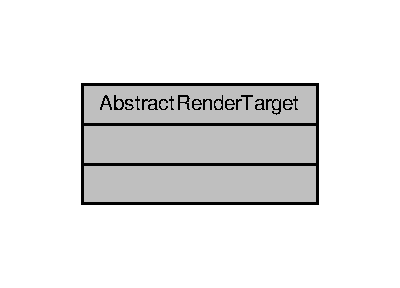
\includegraphics[width=192pt]{class_abstract_render_target__coll__graph}
\end{center}
\end{figure}


\subsection{Detailed Description}
Abstract base class for Open\-G\-L Objects. 

\begin{DoxyAuthor}{Author}
Declan Russell 
\end{DoxyAuthor}
\begin{DoxyDate}{Date}
28/04/2015 
\end{DoxyDate}
\begin{DoxyVersion}{Version}
1.\-0 
\end{DoxyVersion}


The documentation for this class was generated from the following file\-:\begin{DoxyCompactItemize}
\item 
/home/dexternation/\-A\-G\-S\-D\-T\-Fluid\-Sim/include/Abstract\-Open\-G\-L\-Object.\-h\end{DoxyCompactItemize}

\input{class_camera}
\input{struct_text_1_1_font_char}
\hypertarget{class_frame_buffer}{\section{Frame\-Buffer Class Reference}
\label{class_frame_buffer}\index{Frame\-Buffer@{Frame\-Buffer}}
}


Class for creating frame buffers.  




{\ttfamily \#include $<$Frame\-Buffer.\-h$>$}



Inheritance diagram for Frame\-Buffer\-:


Collaboration diagram for Frame\-Buffer\-:
\subsection*{Public Member Functions}
\begin{DoxyCompactItemize}
\item 
\hypertarget{class_frame_buffer_a6f3763f4551f221b86ca033e2b315c42}{\hyperlink{class_frame_buffer_a6f3763f4551f221b86ca033e2b315c42}{Frame\-Buffer} ()}\label{class_frame_buffer_a6f3763f4551f221b86ca033e2b315c42}

\begin{DoxyCompactList}\small\item\em default constructor to create our frame buffer \end{DoxyCompactList}\item 
\hypertarget{class_frame_buffer_aef8be9884e8cc0fc3f3692e6c6968fa1}{\hyperlink{class_frame_buffer_aef8be9884e8cc0fc3f3692e6c6968fa1}{$\sim$\-Frame\-Buffer} ()}\label{class_frame_buffer_aef8be9884e8cc0fc3f3692e6c6968fa1}

\begin{DoxyCompactList}\small\item\em default destructor removes frambuffers \end{DoxyCompactList}\item 
\hypertarget{class_frame_buffer_a16fa30984714c6070f4c5bde5b5b87f7}{void \hyperlink{class_frame_buffer_a16fa30984714c6070f4c5bde5b5b87f7}{bind} ()}\label{class_frame_buffer_a16fa30984714c6070f4c5bde5b5b87f7}

\begin{DoxyCompactList}\small\item\em bind our frame buffer \end{DoxyCompactList}\item 
\hypertarget{class_frame_buffer_a3b82af89f1c0c0f4c0140e41863256c0}{void \hyperlink{class_frame_buffer_a3b82af89f1c0c0f4c0140e41863256c0}{unbind} ()}\label{class_frame_buffer_a3b82af89f1c0c0f4c0140e41863256c0}

\begin{DoxyCompactList}\small\item\em unbind our frame buffer \end{DoxyCompactList}\item 
\hypertarget{class_frame_buffer_a3acf3a4afec2ebecd93fae3bfba00808}{void \hyperlink{class_frame_buffer_a3acf3a4afec2ebecd93fae3bfba00808}{set\-Frame\-Buffer\-Texture} (G\-Lenum \-\_\-attachment, G\-Luint \-\_\-texture, G\-Lint \-\_\-level)}\label{class_frame_buffer_a3acf3a4afec2ebecd93fae3bfba00808}

\begin{DoxyCompactList}\small\item\em set our frame buffer texture \end{DoxyCompactList}\item 
\hypertarget{class_frame_buffer_a399edc3b7d856ead72e5e04d73223643}{void \hyperlink{class_frame_buffer_a399edc3b7d856ead72e5e04d73223643}{set\-Drawbuffers} (G\-Lsizei \-\_\-n, const G\-Lenum $\ast$\-\_\-bufs)}\label{class_frame_buffer_a399edc3b7d856ead72e5e04d73223643}

\begin{DoxyCompactList}\small\item\em set the draw buffers of our frame buffer \end{DoxyCompactList}\end{DoxyCompactItemize}
\subsection*{Additional Inherited Members}


\subsection{Detailed Description}
Class for creating frame buffers. 

\begin{DoxyAuthor}{Author}
Declan Russell 
\end{DoxyAuthor}
\begin{DoxyDate}{Date}
28/04/2015 
\end{DoxyDate}
\begin{DoxyVersion}{Version}
1.\-0 
\end{DoxyVersion}


The documentation for this class was generated from the following files\-:\begin{DoxyCompactItemize}
\item 
include/\hyperlink{_frame_buffer_8h}{Frame\-Buffer.\-h}\item 
src/Frame\-Buffer.\-cpp\end{DoxyCompactItemize}

\hypertarget{class_g_l_texture}{\section{G\-L\-Texture Class Reference}
\label{class_g_l_texture}\index{G\-L\-Texture@{G\-L\-Texture}}
}


Inheritance diagram for G\-L\-Texture\-:\nopagebreak
\begin{figure}[H]
\begin{center}
\leavevmode
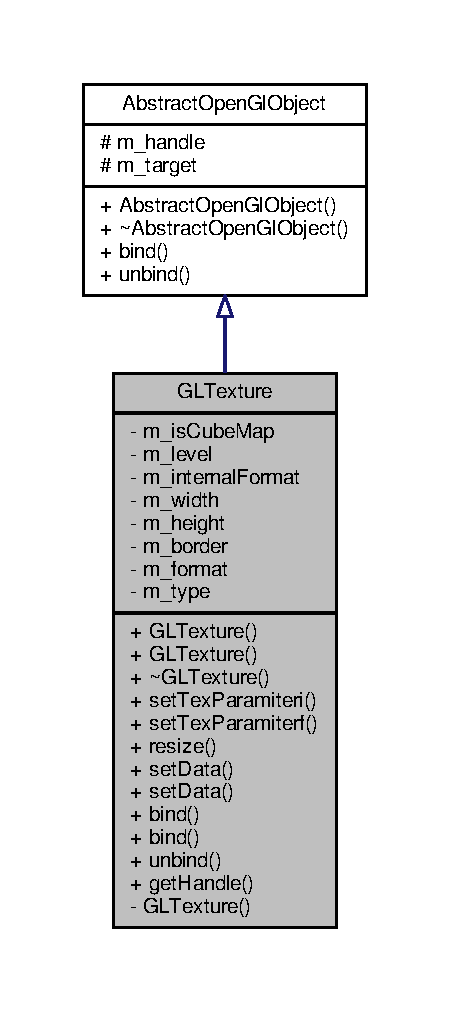
\includegraphics[width=216pt]{class_g_l_texture__inherit__graph}
\end{center}
\end{figure}


Collaboration diagram for G\-L\-Texture\-:\nopagebreak
\begin{figure}[H]
\begin{center}
\leavevmode
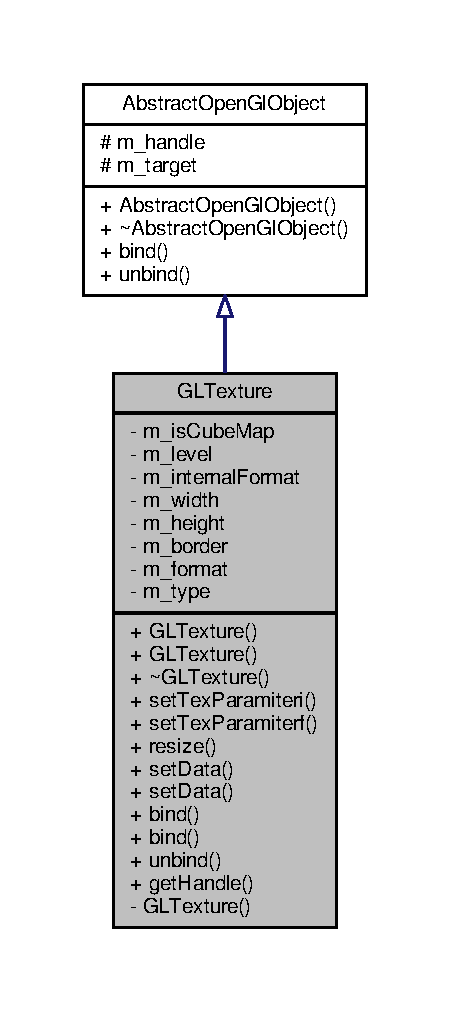
\includegraphics[width=216pt]{class_g_l_texture__coll__graph}
\end{center}
\end{figure}
\subsection*{Public Member Functions}
\begin{DoxyCompactItemize}
\item 
\hyperlink{class_g_l_texture_a1f0c33b32b1e37985976b6f10c2263c3}{G\-L\-Texture} (G\-Lenum \-\_\-target, G\-Lint \-\_\-level, G\-Lint \-\_\-internal\-Format, G\-Lsizei \-\_\-width, G\-Lsizei \-\_\-height, G\-Lint \-\_\-border, G\-Lenum \-\_\-format, G\-Lenum \-\_\-type, const G\-Lvoid $\ast$\-\_\-data)
\begin{DoxyCompactList}\small\item\em Constructor that creates our texture on our G\-P\-U. \end{DoxyCompactList}\item 
\hyperlink{class_g_l_texture_a0ec835c5a25261ce08b43b7a1601fc8f}{G\-L\-Texture} (G\-Lenum \-\_\-target, G\-Lint \-\_\-level, G\-Lint \-\_\-internal\-Format, G\-Lsizei \-\_\-width, G\-Lsizei \-\_\-height, G\-Lint \-\_\-border, G\-Lenum \-\_\-format, G\-Lenum \-\_\-type, const G\-Lvoid $\ast$\-\_\-front, const G\-Lvoid $\ast$\-\_\-back, const G\-Lvoid $\ast$\-\_\-top, const G\-Lvoid $\ast$\-\_\-bottom, const G\-Lvoid $\ast$\-\_\-left, const G\-Lvoid $\ast$\-\_\-right)
\begin{DoxyCompactList}\small\item\em Constructor that creates a cube map texture on our G\-P\-U. \end{DoxyCompactList}\item 
\hypertarget{class_g_l_texture_a7a0f04b3bd68c77588c0aea9b30b08c4}{\hyperlink{class_g_l_texture_a7a0f04b3bd68c77588c0aea9b30b08c4}{$\sim$\-G\-L\-Texture} ()}\label{class_g_l_texture_a7a0f04b3bd68c77588c0aea9b30b08c4}

\begin{DoxyCompactList}\small\item\em our destrutor that removes our texture \end{DoxyCompactList}\item 
\hypertarget{class_g_l_texture_add43b53521541bad76faec1cc5292048}{void \hyperlink{class_g_l_texture_add43b53521541bad76faec1cc5292048}{set\-Tex\-Paramiteri} (G\-Lenum \-\_\-pname, G\-Lint \-\_\-param)}\label{class_g_l_texture_add43b53521541bad76faec1cc5292048}

\begin{DoxyCompactList}\small\item\em set our texture integer paramiters same as gl\-Tex\-Paramiteri see Open\-G\-L documentation for more info \end{DoxyCompactList}\item 
\hypertarget{class_g_l_texture_a2a2d0c69601ba7843dd33def3f0d28a2}{void \hyperlink{class_g_l_texture_a2a2d0c69601ba7843dd33def3f0d28a2}{set\-Tex\-Paramiterf} (G\-Lenum \-\_\-pname, G\-Lfloat \-\_\-param)}\label{class_g_l_texture_a2a2d0c69601ba7843dd33def3f0d28a2}

\begin{DoxyCompactList}\small\item\em set our texture float paramiters same as gl\-Tex\-Paramiterf see Open\-G\-L documentation for more info \end{DoxyCompactList}\item 
void \hyperlink{class_g_l_texture_a5b70c5df1d184c9be005b0ed05f1e808}{resize} (G\-Lsizei \-\_\-width, G\-Lsizei \-\_\-height=0)
\begin{DoxyCompactList}\small\item\em resizes our texture \end{DoxyCompactList}\item 
void \hyperlink{class_g_l_texture_a9214dfefb40db4fbb7450bcc0ba70b61}{set\-Data} (const G\-Lvoid $\ast$\-\_\-data, G\-Lsizei \-\_\-width=-\/1, G\-Lsizei \-\_\-height=-\/1)
\begin{DoxyCompactList}\small\item\em set the data of our textue \end{DoxyCompactList}\item 
\hypertarget{class_g_l_texture_af20871f52b9705409078558a33a2c73d}{void \hyperlink{class_g_l_texture_af20871f52b9705409078558a33a2c73d}{set\-Data} (const G\-Lvoid $\ast$\-\_\-front, const G\-Lvoid $\ast$\-\_\-back, const G\-Lvoid $\ast$\-\_\-top, const G\-Lvoid $\ast$\-\_\-bottom, const G\-Lvoid $\ast$\-\_\-left, const G\-Lvoid $\ast$\-\_\-right, G\-Lsizei \-\_\-width=-\/1, G\-Lsizei \-\_\-height=-\/1)}\label{class_g_l_texture_af20871f52b9705409078558a33a2c73d}

\begin{DoxyCompactList}\small\item\em set the data for a cube map texture \end{DoxyCompactList}\item 
void \hyperlink{class_g_l_texture_a8fcf4e5253bccd04ffe6e65af228dabc}{bind} (unsigned int \-\_\-loc)
\begin{DoxyCompactList}\small\item\em binds our texture and set active texture \end{DoxyCompactList}\item 
\hypertarget{class_g_l_texture_a3d26fc3a017fd2079ab67e422f9bac10}{void \hyperlink{class_g_l_texture_a3d26fc3a017fd2079ab67e422f9bac10}{bind} ()}\label{class_g_l_texture_a3d26fc3a017fd2079ab67e422f9bac10}

\begin{DoxyCompactList}\small\item\em binds our texture \end{DoxyCompactList}\item 
\hypertarget{class_g_l_texture_a96090b31b8d550a50eb1d4bed1055774}{void \hyperlink{class_g_l_texture_a96090b31b8d550a50eb1d4bed1055774}{unbind} ()}\label{class_g_l_texture_a96090b31b8d550a50eb1d4bed1055774}

\begin{DoxyCompactList}\small\item\em unbinds our texture \end{DoxyCompactList}\item 
\hypertarget{class_g_l_texture_a0232aa38a299d2570a06367cd8ebd688}{G\-Luint \hyperlink{class_g_l_texture_a0232aa38a299d2570a06367cd8ebd688}{get\-Handle} ()}\label{class_g_l_texture_a0232aa38a299d2570a06367cd8ebd688}

\begin{DoxyCompactList}\small\item\em accessor to the handle of our texture \end{DoxyCompactList}\end{DoxyCompactItemize}
\subsection*{Private Member Functions}
\begin{DoxyCompactItemize}
\item 
\hypertarget{class_g_l_texture_abb3da94e96ea6893e33e51c5422a42f9}{\hyperlink{class_g_l_texture_abb3da94e96ea6893e33e51c5422a42f9}{G\-L\-Texture} ()}\label{class_g_l_texture_abb3da94e96ea6893e33e51c5422a42f9}

\begin{DoxyCompactList}\small\item\em default construtor never to be used. \end{DoxyCompactList}\end{DoxyCompactItemize}
\subsection*{Private Attributes}
\begin{DoxyCompactItemize}
\item 
\hypertarget{class_g_l_texture_afd2e590d7242b2ab54d0ac1473ada6cb}{bool \hyperlink{class_g_l_texture_afd2e590d7242b2ab54d0ac1473ada6cb}{m\-\_\-is\-Cube\-Map}}\label{class_g_l_texture_afd2e590d7242b2ab54d0ac1473ada6cb}

\begin{DoxyCompactList}\small\item\em bool to define if our texture is a cube map \end{DoxyCompactList}\item 
\hypertarget{class_g_l_texture_a7add2254b205660a18801f3e9df6d2b9}{G\-Lint \hyperlink{class_g_l_texture_a7add2254b205660a18801f3e9df6d2b9}{m\-\_\-level}}\label{class_g_l_texture_a7add2254b205660a18801f3e9df6d2b9}

\begin{DoxyCompactList}\small\item\em L\-O\-D detail number. \end{DoxyCompactList}\item 
\hypertarget{class_g_l_texture_a1298a4da5241c3f08188a91efdc820a3}{G\-Lint \hyperlink{class_g_l_texture_a1298a4da5241c3f08188a91efdc820a3}{m\-\_\-internal\-Format}}\label{class_g_l_texture_a1298a4da5241c3f08188a91efdc820a3}

\begin{DoxyCompactList}\small\item\em internal format \end{DoxyCompactList}\item 
\hypertarget{class_g_l_texture_ae2f00682c8694bd9ba1d348363f115f4}{G\-Lsizei \hyperlink{class_g_l_texture_ae2f00682c8694bd9ba1d348363f115f4}{m\-\_\-width}}\label{class_g_l_texture_ae2f00682c8694bd9ba1d348363f115f4}

\begin{DoxyCompactList}\small\item\em width of our texture \end{DoxyCompactList}\item 
\hypertarget{class_g_l_texture_a5148727b47ef344338fad34d8ae9c06c}{G\-Lsizei \hyperlink{class_g_l_texture_a5148727b47ef344338fad34d8ae9c06c}{m\-\_\-height}}\label{class_g_l_texture_a5148727b47ef344338fad34d8ae9c06c}

\begin{DoxyCompactList}\small\item\em height of our texture \end{DoxyCompactList}\item 
\hypertarget{class_g_l_texture_a3a568e28bbc01e1adb7cf33f6889bce5}{G\-Lint \hyperlink{class_g_l_texture_a3a568e28bbc01e1adb7cf33f6889bce5}{m\-\_\-border}}\label{class_g_l_texture_a3a568e28bbc01e1adb7cf33f6889bce5}

\begin{DoxyCompactList}\small\item\em border size of our texture \end{DoxyCompactList}\item 
\hypertarget{class_g_l_texture_af2812d7eebea9c63a59e2994a745e8d0}{G\-Lenum \hyperlink{class_g_l_texture_af2812d7eebea9c63a59e2994a745e8d0}{m\-\_\-format}}\label{class_g_l_texture_af2812d7eebea9c63a59e2994a745e8d0}

\begin{DoxyCompactList}\small\item\em format of our texture \end{DoxyCompactList}\item 
\hypertarget{class_g_l_texture_a1f9a5c5d3ed73c2b2ad6be52967fd883}{G\-Lenum \hyperlink{class_g_l_texture_a1f9a5c5d3ed73c2b2ad6be52967fd883}{m\-\_\-type}}\label{class_g_l_texture_a1f9a5c5d3ed73c2b2ad6be52967fd883}

\begin{DoxyCompactList}\small\item\em type of pixel data \end{DoxyCompactList}\end{DoxyCompactItemize}
\subsection*{Additional Inherited Members}


\subsection{Constructor \& Destructor Documentation}
\hypertarget{class_g_l_texture_a1f0c33b32b1e37985976b6f10c2263c3}{\index{G\-L\-Texture@{G\-L\-Texture}!G\-L\-Texture@{G\-L\-Texture}}
\index{G\-L\-Texture@{G\-L\-Texture}!GLTexture@{G\-L\-Texture}}
\subsubsection[{G\-L\-Texture}]{\setlength{\rightskip}{0pt plus 5cm}G\-L\-Texture\-::\-G\-L\-Texture (
\begin{DoxyParamCaption}
\item[{G\-Lenum}]{\-\_\-target, }
\item[{G\-Lint}]{\-\_\-level, }
\item[{G\-Lint}]{\-\_\-internal\-Format, }
\item[{G\-Lsizei}]{\-\_\-width, }
\item[{G\-Lsizei}]{\-\_\-height, }
\item[{G\-Lint}]{\-\_\-border, }
\item[{G\-Lenum}]{\-\_\-format, }
\item[{G\-Lenum}]{\-\_\-type, }
\item[{const G\-Lvoid $\ast$}]{\-\_\-data}
\end{DoxyParamCaption}
)}}\label{class_g_l_texture_a1f0c33b32b1e37985976b6f10c2263c3}


Constructor that creates our texture on our G\-P\-U. 

See Open\-G\-L documentation for detail about texture paramiters 

Here is the call graph for this function\-:\nopagebreak
\begin{figure}[H]
\begin{center}
\leavevmode
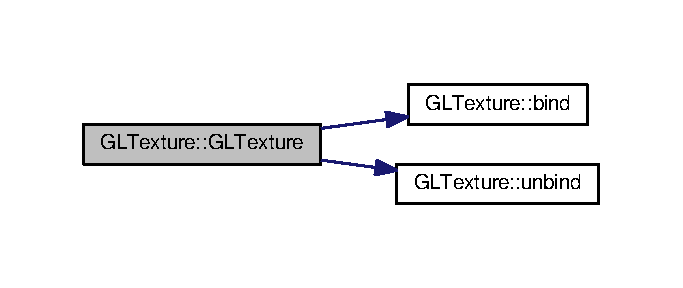
\includegraphics[width=328pt]{class_g_l_texture_a1f0c33b32b1e37985976b6f10c2263c3_cgraph}
\end{center}
\end{figure}


\hypertarget{class_g_l_texture_a0ec835c5a25261ce08b43b7a1601fc8f}{\index{G\-L\-Texture@{G\-L\-Texture}!G\-L\-Texture@{G\-L\-Texture}}
\index{G\-L\-Texture@{G\-L\-Texture}!GLTexture@{G\-L\-Texture}}
\subsubsection[{G\-L\-Texture}]{\setlength{\rightskip}{0pt plus 5cm}G\-L\-Texture\-::\-G\-L\-Texture (
\begin{DoxyParamCaption}
\item[{G\-Lenum}]{\-\_\-target, }
\item[{G\-Lint}]{\-\_\-level, }
\item[{G\-Lint}]{\-\_\-internal\-Format, }
\item[{G\-Lsizei}]{\-\_\-width, }
\item[{G\-Lsizei}]{\-\_\-height, }
\item[{G\-Lint}]{\-\_\-border, }
\item[{G\-Lenum}]{\-\_\-format, }
\item[{G\-Lenum}]{\-\_\-type, }
\item[{const G\-Lvoid $\ast$}]{\-\_\-front, }
\item[{const G\-Lvoid $\ast$}]{\-\_\-back, }
\item[{const G\-Lvoid $\ast$}]{\-\_\-top, }
\item[{const G\-Lvoid $\ast$}]{\-\_\-bottom, }
\item[{const G\-Lvoid $\ast$}]{\-\_\-left, }
\item[{const G\-Lvoid $\ast$}]{\-\_\-right}
\end{DoxyParamCaption}
)}}\label{class_g_l_texture_a0ec835c5a25261ce08b43b7a1601fc8f}


Constructor that creates a cube map texture on our G\-P\-U. 

See Open\-G\-L documentation for detail about texture paramiters 

Here is the call graph for this function\-:\nopagebreak
\begin{figure}[H]
\begin{center}
\leavevmode
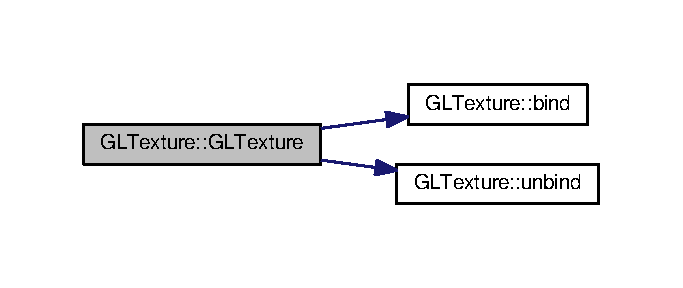
\includegraphics[width=328pt]{class_g_l_texture_a0ec835c5a25261ce08b43b7a1601fc8f_cgraph}
\end{center}
\end{figure}




\subsection{Member Function Documentation}
\hypertarget{class_g_l_texture_a8fcf4e5253bccd04ffe6e65af228dabc}{\index{G\-L\-Texture@{G\-L\-Texture}!bind@{bind}}
\index{bind@{bind}!GLTexture@{G\-L\-Texture}}
\subsubsection[{bind}]{\setlength{\rightskip}{0pt plus 5cm}void G\-L\-Texture\-::bind (
\begin{DoxyParamCaption}
\item[{unsigned int}]{\-\_\-loc}
\end{DoxyParamCaption}
)}}\label{class_g_l_texture_a8fcf4e5253bccd04ffe6e65af228dabc}


binds our texture and set active texture 


\begin{DoxyParams}{Parameters}
{\em \-\_\-loc} & -\/ active texture location to bind to \\
\hline
\end{DoxyParams}
\hypertarget{class_g_l_texture_a5b70c5df1d184c9be005b0ed05f1e808}{\index{G\-L\-Texture@{G\-L\-Texture}!resize@{resize}}
\index{resize@{resize}!GLTexture@{G\-L\-Texture}}
\subsubsection[{resize}]{\setlength{\rightskip}{0pt plus 5cm}void G\-L\-Texture\-::resize (
\begin{DoxyParamCaption}
\item[{G\-Lsizei}]{\-\_\-width, }
\item[{G\-Lsizei}]{\-\_\-height = {\ttfamily 0}}
\end{DoxyParamCaption}
)}}\label{class_g_l_texture_a5b70c5df1d184c9be005b0ed05f1e808}


resizes our texture 


\begin{DoxyParams}{Parameters}
{\em \-\_\-width} & -\/ width to resize texture \\
\hline
{\em \-\_\-height} & -\/ height to resize texture \\
\hline
\end{DoxyParams}


Here is the call graph for this function\-:\nopagebreak
\begin{figure}[H]
\begin{center}
\leavevmode
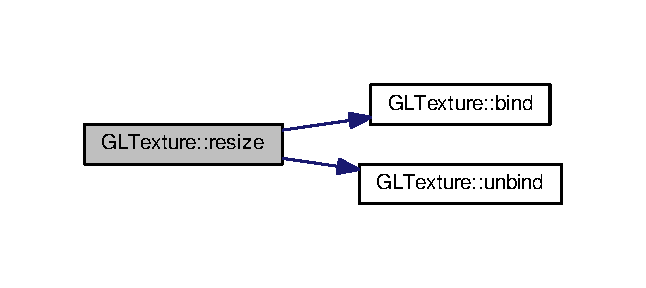
\includegraphics[width=310pt]{class_g_l_texture_a5b70c5df1d184c9be005b0ed05f1e808_cgraph}
\end{center}
\end{figure}


\hypertarget{class_g_l_texture_a9214dfefb40db4fbb7450bcc0ba70b61}{\index{G\-L\-Texture@{G\-L\-Texture}!set\-Data@{set\-Data}}
\index{set\-Data@{set\-Data}!GLTexture@{G\-L\-Texture}}
\subsubsection[{set\-Data}]{\setlength{\rightskip}{0pt plus 5cm}void G\-L\-Texture\-::set\-Data (
\begin{DoxyParamCaption}
\item[{const G\-Lvoid $\ast$}]{\-\_\-data, }
\item[{G\-Lsizei}]{\-\_\-width = {\ttfamily -\/1}, }
\item[{G\-Lsizei}]{\-\_\-height = {\ttfamily -\/1}}
\end{DoxyParamCaption}
)}}\label{class_g_l_texture_a9214dfefb40db4fbb7450bcc0ba70b61}


set the data of our textue 


\begin{DoxyParams}{Parameters}
{\em \-\_\-data} & -\/ data to set to texture \\
\hline
\end{DoxyParams}


Here is the call graph for this function\-:\nopagebreak
\begin{figure}[H]
\begin{center}
\leavevmode
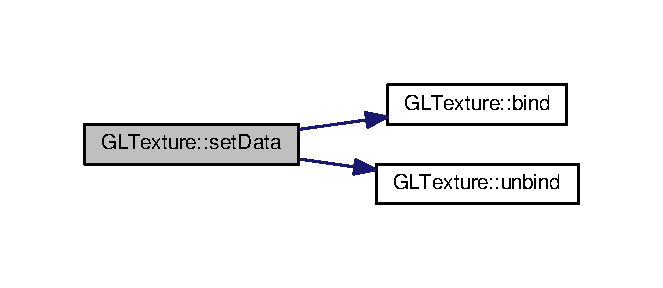
\includegraphics[width=318pt]{class_g_l_texture_a9214dfefb40db4fbb7450bcc0ba70b61_cgraph}
\end{center}
\end{figure}




The documentation for this class was generated from the following files\-:\begin{DoxyCompactItemize}
\item 
/home/dexternation/\-A\-G\-S\-D\-T\-Fluid\-Sim/include/\hyperlink{_g_l_texture_8h}{G\-L\-Texture.\-h}\item 
/home/dexternation/\-A\-G\-S\-D\-T\-Fluid\-Sim/src/G\-L\-Texture.\-cpp\end{DoxyCompactItemize}

\hypertarget{class_g_l_texture_lib}{\section{G\-L\-Texture\-Lib Class Reference}
\label{class_g_l_texture_lib}\index{G\-L\-Texture\-Lib@{G\-L\-Texture\-Lib}}
}


Simple class for loading in and managing Open\-G\-L textures.  




{\ttfamily \#include $<$G\-L\-Texture.\-h$>$}



Collaboration diagram for G\-L\-Texture\-Lib\-:
\subsection*{Public Member Functions}
\begin{DoxyCompactItemize}
\item 
\hyperlink{class_g_l_texture}{G\-L\-Texture} $\ast$ \hyperlink{class_g_l_texture_lib_a778cde3734906f46649defdda30d7d7e}{add\-Texture} (std\-::string \-\_\-name, G\-Lenum \-\_\-target, G\-Lint \-\_\-level, G\-Lint \-\_\-internal\-Format, G\-Lsizei \-\_\-width, G\-Lsizei \-\_\-height, G\-Lint \-\_\-border, G\-Lenum \-\_\-format, G\-Lenum \-\_\-type, const G\-Lvoid $\ast$\-\_\-data)
\begin{DoxyCompactList}\small\item\em add a texture to our texture library \end{DoxyCompactList}\item 
\hyperlink{class_g_l_texture}{G\-L\-Texture} $\ast$ \hyperlink{class_g_l_texture_lib_aece253fdd6aad02adca2d743c463a9f2}{add\-Cube\-Map} (std\-::string \-\_\-name, G\-Lenum \-\_\-target, G\-Lint \-\_\-level, G\-Lint \-\_\-internal\-Format, G\-Lsizei \-\_\-width, G\-Lsizei \-\_\-height, G\-Lint \-\_\-border, G\-Lenum \-\_\-format, G\-Lenum \-\_\-type, const G\-Lvoid $\ast$\-\_\-front, const G\-Lvoid $\ast$\-\_\-back, const G\-Lvoid $\ast$\-\_\-top, const G\-Lvoid $\ast$\-\_\-bottom, const G\-Lvoid $\ast$\-\_\-left, const G\-Lvoid $\ast$\-\_\-right)
\begin{DoxyCompactList}\small\item\em add a cube map to our texture library \end{DoxyCompactList}\item 
\hypertarget{class_g_l_texture_lib_aa18a039ee29d50ccd34a7e1f7d24ce5b}{\hyperlink{class_g_l_texture}{G\-L\-Texture} $\ast$ \hyperlink{class_g_l_texture_lib_aa18a039ee29d50ccd34a7e1f7d24ce5b}{operator\mbox{[}$\,$\mbox{]}} (const std\-::string \&\-\_\-name)}\label{class_g_l_texture_lib_aa18a039ee29d50ccd34a7e1f7d24ce5b}

\begin{DoxyCompactList}\small\item\em overloaded operators to access a texture in our library \end{DoxyCompactList}\item 
\hypertarget{class_g_l_texture_lib_ab4ab9d6def1eb2acecfbe062686ab98e}{\hyperlink{class_g_l_texture}{G\-L\-Texture} $\ast$ \hyperlink{class_g_l_texture_lib_ab4ab9d6def1eb2acecfbe062686ab98e}{operator\mbox{[}$\,$\mbox{]}} (const char $\ast$\-\_\-name)}\label{class_g_l_texture_lib_ab4ab9d6def1eb2acecfbe062686ab98e}

\begin{DoxyCompactList}\small\item\em overloaded operators to access a texture in our library \end{DoxyCompactList}\item 
\hypertarget{class_g_l_texture_lib_aca4b2bd67c1af5b5c1ea304fe2622eac}{\hyperlink{class_g_l_texture_lib_aca4b2bd67c1af5b5c1ea304fe2622eac}{$\sim$\-G\-L\-Texture\-Lib} ()}\label{class_g_l_texture_lib_aca4b2bd67c1af5b5c1ea304fe2622eac}

\begin{DoxyCompactList}\small\item\em our destructor. Removes all textures from library \end{DoxyCompactList}\item 
\hypertarget{class_g_l_texture_lib_a49ba9410297b15f1f2988369853c108f}{void \hyperlink{class_g_l_texture_lib_a49ba9410297b15f1f2988369853c108f}{destroy} ()}\label{class_g_l_texture_lib_a49ba9410297b15f1f2988369853c108f}

\begin{DoxyCompactList}\small\item\em Deletes our library. \end{DoxyCompactList}\end{DoxyCompactItemize}
\subsection*{Static Public Member Functions}
\begin{DoxyCompactItemize}
\item 
\hypertarget{class_g_l_texture_lib_aedb1360fe37f369eb290f773dbada309}{static \hyperlink{class_g_l_texture_lib}{G\-L\-Texture\-Lib} $\ast$ \hyperlink{class_g_l_texture_lib_aedb1360fe37f369eb290f773dbada309}{get\-Instance} ()}\label{class_g_l_texture_lib_aedb1360fe37f369eb290f773dbada309}

\begin{DoxyCompactList}\small\item\em returns an instance of our texture library \end{DoxyCompactList}\end{DoxyCompactItemize}
\subsection*{Private Member Functions}
\begin{DoxyCompactItemize}
\item 
\hypertarget{class_g_l_texture_lib_a7ac1f52801de2e75472f3bd495c40185}{\hyperlink{class_g_l_texture_lib_a7ac1f52801de2e75472f3bd495c40185}{G\-L\-Texture\-Lib} ()}\label{class_g_l_texture_lib_a7ac1f52801de2e75472f3bd495c40185}

\begin{DoxyCompactList}\small\item\em our default constructor. Don't want this to be accessable as this is a singleton class \end{DoxyCompactList}\end{DoxyCompactItemize}
\subsection*{Private Attributes}
\begin{DoxyCompactItemize}
\item 
\hypertarget{class_g_l_texture_lib_a148bbba73a37d5478e1f037699f51d94}{\hyperlink{class_g_l_texture}{G\-L\-Texture} $\ast$ \hyperlink{class_g_l_texture_lib_a148bbba73a37d5478e1f037699f51d94}{m\-\_\-current\-Texture}}\label{class_g_l_texture_lib_a148bbba73a37d5478e1f037699f51d94}

\begin{DoxyCompactList}\small\item\em the current texture in use \end{DoxyCompactList}\item 
\hypertarget{class_g_l_texture_lib_a931a6e49b5a86564de11359436dfb745}{std\-::string \hyperlink{class_g_l_texture_lib_a931a6e49b5a86564de11359436dfb745}{m\-\_\-current\-Texture\-Name}}\label{class_g_l_texture_lib_a931a6e49b5a86564de11359436dfb745}

\begin{DoxyCompactList}\small\item\em the current texture in use name \end{DoxyCompactList}\item 
\hypertarget{class_g_l_texture_lib_adbacf6d620b239b381e955ef4277a6a6}{std\-::map$<$ std\-::string, \\*
\hyperlink{class_g_l_texture}{G\-L\-Texture} $\ast$ $>$ \hyperlink{class_g_l_texture_lib_adbacf6d620b239b381e955ef4277a6a6}{m\-\_\-textures}}\label{class_g_l_texture_lib_adbacf6d620b239b381e955ef4277a6a6}

\begin{DoxyCompactList}\small\item\em mip map for storing our textures \end{DoxyCompactList}\end{DoxyCompactItemize}
\subsection*{Static Private Attributes}
\begin{DoxyCompactItemize}
\item 
\hypertarget{class_g_l_texture_lib_a54710e7dffef1a0d7e383802298c5c3a}{static \hyperlink{class_g_l_texture_lib}{G\-L\-Texture\-Lib} $\ast$ \hyperlink{class_g_l_texture_lib_a54710e7dffef1a0d7e383802298c5c3a}{m\-\_\-instance}}\label{class_g_l_texture_lib_a54710e7dffef1a0d7e383802298c5c3a}

\begin{DoxyCompactList}\small\item\em our static instance of our texture library \end{DoxyCompactList}\end{DoxyCompactItemize}


\subsection{Detailed Description}
Simple class for loading in and managing Open\-G\-L textures. 

Singleton class for creating and storing textures in a library.

\begin{DoxyAuthor}{Author}
Declan Russell 
\end{DoxyAuthor}
\begin{DoxyDate}{Date}
28/04/2015 
\end{DoxyDate}
\begin{DoxyVersion}{Version}
1.\-0 
\end{DoxyVersion}


\subsection{Member Function Documentation}
\hypertarget{class_g_l_texture_lib_aece253fdd6aad02adca2d743c463a9f2}{\index{G\-L\-Texture\-Lib@{G\-L\-Texture\-Lib}!add\-Cube\-Map@{add\-Cube\-Map}}
\index{add\-Cube\-Map@{add\-Cube\-Map}!GLTextureLib@{G\-L\-Texture\-Lib}}
\subsubsection[{add\-Cube\-Map}]{\setlength{\rightskip}{0pt plus 5cm}{\bf G\-L\-Texture} $\ast$ G\-L\-Texture\-Lib\-::add\-Cube\-Map (
\begin{DoxyParamCaption}
\item[{std\-::string}]{\-\_\-name, }
\item[{G\-Lenum}]{\-\_\-target, }
\item[{G\-Lint}]{\-\_\-level, }
\item[{G\-Lint}]{\-\_\-internal\-Format, }
\item[{G\-Lsizei}]{\-\_\-width, }
\item[{G\-Lsizei}]{\-\_\-height, }
\item[{G\-Lint}]{\-\_\-border, }
\item[{G\-Lenum}]{\-\_\-format, }
\item[{G\-Lenum}]{\-\_\-type, }
\item[{const G\-Lvoid $\ast$}]{\-\_\-front, }
\item[{const G\-Lvoid $\ast$}]{\-\_\-back, }
\item[{const G\-Lvoid $\ast$}]{\-\_\-top, }
\item[{const G\-Lvoid $\ast$}]{\-\_\-bottom, }
\item[{const G\-Lvoid $\ast$}]{\-\_\-left, }
\item[{const G\-Lvoid $\ast$}]{\-\_\-right}
\end{DoxyParamCaption}
)}}\label{class_g_l_texture_lib_aece253fdd6aad02adca2d743c463a9f2}


add a cube map to our texture library 


\begin{DoxyParams}{Parameters}
{\em \-\_\-name} & -\/ the name of our texture \\
\hline
\end{DoxyParams}
\hypertarget{class_g_l_texture_lib_a778cde3734906f46649defdda30d7d7e}{\index{G\-L\-Texture\-Lib@{G\-L\-Texture\-Lib}!add\-Texture@{add\-Texture}}
\index{add\-Texture@{add\-Texture}!GLTextureLib@{G\-L\-Texture\-Lib}}
\subsubsection[{add\-Texture}]{\setlength{\rightskip}{0pt plus 5cm}{\bf G\-L\-Texture} $\ast$ G\-L\-Texture\-Lib\-::add\-Texture (
\begin{DoxyParamCaption}
\item[{std\-::string}]{\-\_\-name, }
\item[{G\-Lenum}]{\-\_\-target, }
\item[{G\-Lint}]{\-\_\-level, }
\item[{G\-Lint}]{\-\_\-internal\-Format, }
\item[{G\-Lsizei}]{\-\_\-width, }
\item[{G\-Lsizei}]{\-\_\-height, }
\item[{G\-Lint}]{\-\_\-border, }
\item[{G\-Lenum}]{\-\_\-format, }
\item[{G\-Lenum}]{\-\_\-type, }
\item[{const G\-Lvoid $\ast$}]{\-\_\-data}
\end{DoxyParamCaption}
)}}\label{class_g_l_texture_lib_a778cde3734906f46649defdda30d7d7e}


add a texture to our texture library 


\begin{DoxyParams}{Parameters}
{\em \-\_\-name} & -\/ the name of our texture \\
\hline
\end{DoxyParams}


The documentation for this class was generated from the following files\-:\begin{DoxyCompactItemize}
\item 
include/\hyperlink{_g_l_texture_lib_8h}{G\-L\-Texture\-Lib.\-h}\item 
src/G\-L\-Texture\-Lib.\-cpp\end{DoxyCompactItemize}

\hypertarget{class_ui_1_1_main_window}{\section{Ui\-:\-:Main\-Window Class Reference}
\label{class_ui_1_1_main_window}\index{Ui\-::\-Main\-Window@{Ui\-::\-Main\-Window}}
}


Inheritance diagram for Ui\-:\-:Main\-Window\-:\nopagebreak
\begin{figure}[H]
\begin{center}
\leavevmode
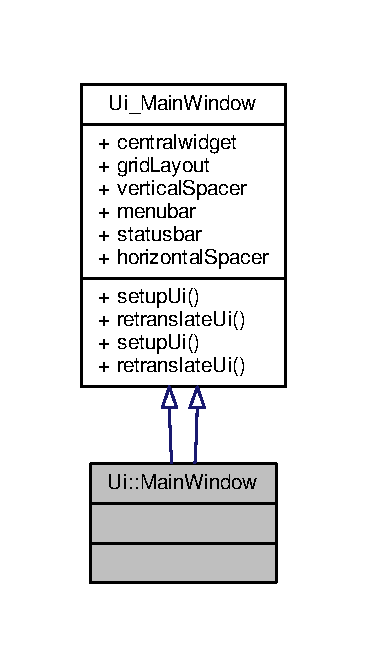
\includegraphics[width=176pt]{class_ui_1_1_main_window__inherit__graph}
\end{center}
\end{figure}


Collaboration diagram for Ui\-:\-:Main\-Window\-:\nopagebreak
\begin{figure}[H]
\begin{center}
\leavevmode
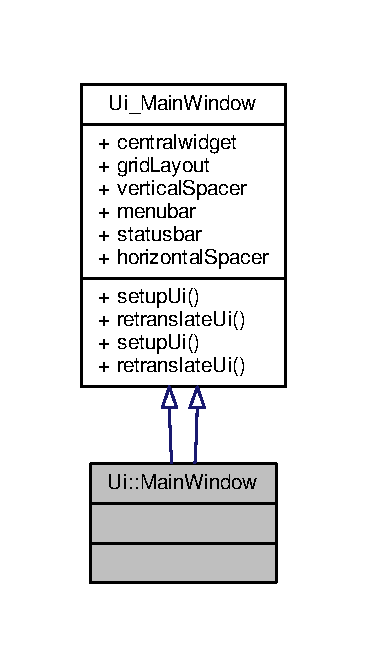
\includegraphics[width=176pt]{class_ui_1_1_main_window__coll__graph}
\end{center}
\end{figure}
\subsection*{Additional Inherited Members}


The documentation for this class was generated from the following file\-:\begin{DoxyCompactItemize}
\item 
/home/dexternation/\-A\-G\-S\-D\-T\-Fluid\-Sim/include/ui\-\_\-mainwindow.\-h\end{DoxyCompactItemize}

\hypertarget{class_main_window}{\section{Main\-Window Class Reference}
\label{class_main_window}\index{Main\-Window@{Main\-Window}}
}


Inheritance diagram for Main\-Window\-:


Collaboration diagram for Main\-Window\-:
\subsection*{Public Slots}
\begin{DoxyCompactItemize}
\item 
\hypertarget{class_main_window_a452fc3db76653e3355cd9eb81bc4f0cf}{void \hyperlink{class_main_window_a452fc3db76653e3355cd9eb81bc4f0cf}{open\-Doc} ()}\label{class_main_window_a452fc3db76653e3355cd9eb81bc4f0cf}

\begin{DoxyCompactList}\small\item\em open documentation slot \end{DoxyCompactList}\end{DoxyCompactItemize}
\subsection*{Public Member Functions}
\begin{DoxyCompactItemize}
\item 
\hypertarget{class_main_window_a8b244be8b7b7db1b08de2a2acb9409db}{{\bfseries Main\-Window} (Q\-Widget $\ast$parent=0)}\label{class_main_window_a8b244be8b7b7db1b08de2a2acb9409db}

\end{DoxyCompactItemize}
\subsection*{Private Attributes}
\begin{DoxyCompactItemize}
\item 
\hypertarget{class_main_window_a35466a70ed47252a0191168126a352a5}{\hyperlink{class_ui_1_1_main_window}{Ui\-::\-Main\-Window} $\ast$ {\bfseries ui}}\label{class_main_window_a35466a70ed47252a0191168126a352a5}

\item 
\hypertarget{class_main_window_af310504f60344259d8a43e495e90e54d}{\hyperlink{class_open_g_l_widget}{Open\-G\-L\-Widget} $\ast$ {\bfseries m\-\_\-open\-G\-L\-Widget}}\label{class_main_window_af310504f60344259d8a43e495e90e54d}

\end{DoxyCompactItemize}


The documentation for this class was generated from the following files\-:\begin{DoxyCompactItemize}
\item 
include/mainwindow.\-h\item 
src/mainwindow.\-cpp\end{DoxyCompactItemize}

\hypertarget{class_open_g_l_widget}{\section{Open\-G\-L\-Widget Class Reference}
\label{class_open_g_l_widget}\index{Open\-G\-L\-Widget@{Open\-G\-L\-Widget}}
}


Basic Qt widget that holds a Open\-G\-L context.  




{\ttfamily \#include $<$Open\-G\-L\-Widget.\-h$>$}



Inheritance diagram for Open\-G\-L\-Widget\-:\nopagebreak
\begin{figure}[H]
\begin{center}
\leavevmode
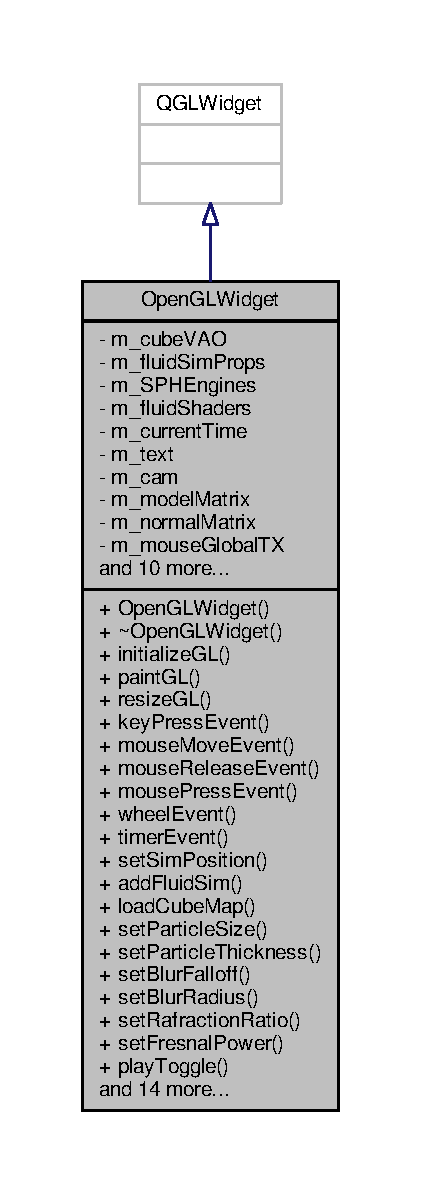
\includegraphics[height=550pt]{class_open_g_l_widget__inherit__graph}
\end{center}
\end{figure}


Collaboration diagram for Open\-G\-L\-Widget\-:\nopagebreak
\begin{figure}[H]
\begin{center}
\leavevmode
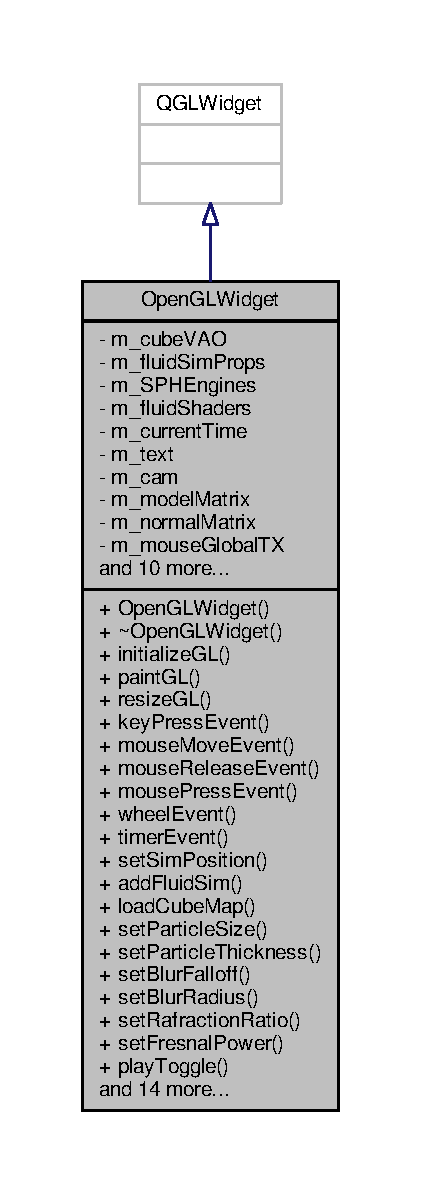
\includegraphics[height=550pt]{class_open_g_l_widget__coll__graph}
\end{center}
\end{figure}
\subsection*{Classes}
\begin{DoxyCompactItemize}
\item 
struct \hyperlink{struct_open_g_l_widget_1_1fluid_sim_props}{fluid\-Sim\-Props}
\begin{DoxyCompactList}\small\item\em structure to hold some update information about our fluid simulations \end{DoxyCompactList}\end{DoxyCompactItemize}
\subsection*{Public Slots}
\begin{DoxyCompactItemize}
\item 
void \hyperlink{class_open_g_l_widget_a6bc6106c82580697f386fdfd2fdb3a12}{set\-Sim\-Position} (float \-\_\-x, float \-\_\-y, float \-\_\-z, int \-\_\-sim\-No=0)
\begin{DoxyCompactList}\small\item\em slot to set sim position \end{DoxyCompactList}\item 
\hypertarget{class_open_g_l_widget_a9ccb72da15f23a16fb74b270a9e19489}{void \hyperlink{class_open_g_l_widget_a9ccb72da15f23a16fb74b270a9e19489}{add\-Fluid\-Sim} ()}\label{class_open_g_l_widget_a9ccb72da15f23a16fb74b270a9e19489}

\begin{DoxyCompactList}\small\item\em slot to add a fluid simulation to our scene \end{DoxyCompactList}\item 
void \hyperlink{class_open_g_l_widget_a39018f8fc74ce591bfac884c277621e6}{load\-Cube\-Map} (Q\-String \-\_\-loc)
\begin{DoxyCompactList}\small\item\em slot to load cube maps to for our enironment map \end{DoxyCompactList}\item 
void \hyperlink{class_open_g_l_widget_a3cdaf60ea4f98ee4782dec21b4810a41}{set\-Particle\-Size} (float \-\_\-size, int \-\_\-sim\-No=0)
\begin{DoxyCompactList}\small\item\em a slot to change our particle size \end{DoxyCompactList}\item 
void \hyperlink{class_open_g_l_widget_aec967838bdff11519892bc05a5d930b0}{set\-Particle\-Thickness} (float \-\_\-thickness, int \-\_\-sim\-No=0)
\begin{DoxyCompactList}\small\item\em a slot to change our particle thickess \end{DoxyCompactList}\item 
void \hyperlink{class_open_g_l_widget_a8e96b44ed40ec8a5fe726f427f01e6fe}{set\-Blur\-Falloff} (float \-\_\-falloff, int \-\_\-sim\-No=0)
\begin{DoxyCompactList}\small\item\em a slot to change our bilateral filter blur falloff \end{DoxyCompactList}\item 
void \hyperlink{class_open_g_l_widget_add467ba5217218564d08ffb638b2f190}{set\-Blur\-Radius} (float \-\_\-radius, int \-\_\-sim\-No=0)
\begin{DoxyCompactList}\small\item\em a slot to change our bilateral filter blur radius \end{DoxyCompactList}\item 
void \hyperlink{class_open_g_l_widget_a9ad49f35e3a76ec5ea58cedbe73afa34}{set\-Rafraction\-Ratio} (float \-\_\-eta, int \-\_\-sim\-No=0)
\begin{DoxyCompactList}\small\item\em a slot to set the refraction ratio of our fluid \end{DoxyCompactList}\item 
void \hyperlink{class_open_g_l_widget_adc34d0b2bed5d7a7f2d5b92fa1b82889}{set\-Fresnal\-Power} (float \-\_\-power, int \-\_\-sim\-No=0)
\begin{DoxyCompactList}\small\item\em a slot to set the fresnal power of our fluid \end{DoxyCompactList}\item 
void \hyperlink{class_open_g_l_widget_a2d1d9bb18d20f1479cb86e832ab17fd2}{play\-Toggle} (int \-\_\-sim\-No=0)
\begin{DoxyCompactList}\small\item\em play/pause toggle slot \end{DoxyCompactList}\item 
void \hyperlink{class_open_g_l_widget_a84585fd40a1fad03bbd118436f5fc477}{set\-Mass} (float \-\_\-mass, int \-\_\-sim\-No=0)
\begin{DoxyCompactList}\small\item\em set volume of our fluid slot \end{DoxyCompactList}\item 
void \hyperlink{class_open_g_l_widget_a785cd8493ea4c1a24a19a16835de4577}{set\-Density} (float \-\_\-den, int \-\_\-sim\-No=0)
\begin{DoxyCompactList}\small\item\em set density of our fluid slot \end{DoxyCompactList}\item 
void \hyperlink{class_open_g_l_widget_aad4c9ceaedc57507d3e9504d15dd8f4a}{set\-Visc\-Coef} (float \-\_\-visc, int \-\_\-sim\-No=0)
\begin{DoxyCompactList}\small\item\em set viscoty coeficient of our fluid slot \end{DoxyCompactList}\item 
void \hyperlink{class_open_g_l_widget_a806e81697e0c6bf0992696ab948bc1c5}{set\-Gas\-Const} (double \-\_\-gas\-Const, int \-\_\-sim\-No=0)
\begin{DoxyCompactList}\small\item\em set gas constant of our fluid slot \end{DoxyCompactList}\item 
void \hyperlink{class_open_g_l_widget_af0f0474b4ff16318e6cf2e7479b369c7}{set\-Smoothing\-Length} (float \-\_\-len, int \-\_\-sim\-No=0)
\begin{DoxyCompactList}\small\item\em set smoothing length of our fluid slot \end{DoxyCompactList}\item 
void \hyperlink{class_open_g_l_widget_a559ba717c412258c234ce5865c0b6976}{set\-Fluid\-Color} (Q\-Color \-\_\-col, int \-\_\-sim\-No=0)
\begin{DoxyCompactList}\small\item\em set the color of our fluid slot \end{DoxyCompactList}\item 
void \hyperlink{class_open_g_l_widget_a3c415ea6ecc1ccf6df49b08df74bbd1a}{set\-Playback\-Speed} (float \-\_\-speed, int \-\_\-sim\-No=0)
\begin{DoxyCompactList}\small\item\em a slot to set the playback speed of our simulation \end{DoxyCompactList}\item 
void \hyperlink{class_open_g_l_widget_ac8a71d325740372032c0061d3bf1daa0}{set\-Sim\-Time\-Step} (float \-\_\-time\-Step, int \-\_\-sim\-No=0)
\begin{DoxyCompactList}\small\item\em a slot to set the time step of our simulation \end{DoxyCompactList}\item 
void \hyperlink{class_open_g_l_widget_acc54210918549bd628db0080d576b483}{reset\-Sim} (int \-\_\-sim\-No)
\begin{DoxyCompactList}\small\item\em a slot to reset our simulation and remove all particles \end{DoxyCompactList}\item 
void \hyperlink{class_open_g_l_widget_ac4d67ea702f268f7d072e94a569cb5f0}{set\-Spawn\-Box\-Position} (float \-\_\-x, float \-\_\-y, float \-\_\-z, int \-\_\-sim\-No=0)
\begin{DoxyCompactList}\small\item\em a slot to set the spawn box position in our simulation \end{DoxyCompactList}\item 
void \hyperlink{class_open_g_l_widget_a60e5e6f2845384c3faeaa11c0fb800b4}{set\-Spawn\-Box\-Size} (float \-\_\-size, int \-\_\-sim\-No=0)
\begin{DoxyCompactList}\small\item\em a slot to set the spawn box size in our simulation \end{DoxyCompactList}\item 
void \hyperlink{class_open_g_l_widget_adce23eb4fa8b5a1d1ac0403c911abb37}{add\-Particles\-To\-Sim} (int \-\_\-num\-Particles, int \-\_\-sim\-No=0)
\begin{DoxyCompactList}\small\item\em slot to add particles to our simulation \end{DoxyCompactList}\item 
void \hyperlink{class_open_g_l_widget_a9ca3397753dcfbc56ada94d1e91000ed}{set\-Vel\-Correction} (float \-\_\-val, int \-\_\-sim\-No=0)
\begin{DoxyCompactList}\small\item\em slot to set the velocity correction of our simulation \end{DoxyCompactList}\item 
void \hyperlink{class_open_g_l_widget_ac4dea29c4b53c1c4906dacd4aa35d975}{set\-Display\-Hud} (bool \-\_\-display, int \-\_\-sim\-No=0)
\begin{DoxyCompactList}\small\item\em slot to toggle display of the hud of our simulatio \end{DoxyCompactList}\end{DoxyCompactItemize}
\subsection*{Public Member Functions}
\begin{DoxyCompactItemize}
\item 
\hyperlink{class_open_g_l_widget_a60b9008fd7762190918d5e2528a57248}{Open\-G\-L\-Widget} (const Q\-G\-L\-Format \-\_\-format, Q\-Widget $\ast$\-\_\-parent=0)
\begin{DoxyCompactList}\small\item\em ctor for our N\-G\-L drawing class \end{DoxyCompactList}\item 
\hypertarget{class_open_g_l_widget_a293847f6a7e6c40344a1acfca3e9eb51}{\hyperlink{class_open_g_l_widget_a293847f6a7e6c40344a1acfca3e9eb51}{$\sim$\-Open\-G\-L\-Widget} ()}\label{class_open_g_l_widget_a293847f6a7e6c40344a1acfca3e9eb51}

\begin{DoxyCompactList}\small\item\em dtor must close down and release Open\-G\-L resources \end{DoxyCompactList}\item 
\hypertarget{class_open_g_l_widget_a570df546f7206455c57addb624906576}{void \hyperlink{class_open_g_l_widget_a570df546f7206455c57addb624906576}{initialize\-G\-L} ()}\label{class_open_g_l_widget_a570df546f7206455c57addb624906576}

\begin{DoxyCompactList}\small\item\em the virtual initialize class is called once when the window is created and we have a valid G\-L context use this to setup any default G\-L stuff \end{DoxyCompactList}\item 
\hypertarget{class_open_g_l_widget_a260a543726f601659cbd1809b90f9e4b}{void \hyperlink{class_open_g_l_widget_a260a543726f601659cbd1809b90f9e4b}{paint\-G\-L} ()}\label{class_open_g_l_widget_a260a543726f601659cbd1809b90f9e4b}

\begin{DoxyCompactList}\small\item\em this is called everytime we want to draw the scene \end{DoxyCompactList}\item 
\hypertarget{class_open_g_l_widget_a55cf4659a7f10207fb6ab3fcf9273abc}{void \hyperlink{class_open_g_l_widget_a55cf4659a7f10207fb6ab3fcf9273abc}{resize\-G\-L} (const int \-\_\-w, const int \-\_\-h)}\label{class_open_g_l_widget_a55cf4659a7f10207fb6ab3fcf9273abc}

\begin{DoxyCompactList}\small\item\em called to resize the window \end{DoxyCompactList}\item 
\hypertarget{class_open_g_l_widget_a2e7ec0372fb6b2a0eb85a9524cfdd7fd}{void \hyperlink{class_open_g_l_widget_a2e7ec0372fb6b2a0eb85a9524cfdd7fd}{key\-Press\-Event} (Q\-Key\-Event $\ast$\-\_\-event)}\label{class_open_g_l_widget_a2e7ec0372fb6b2a0eb85a9524cfdd7fd}

\begin{DoxyCompactList}\small\item\em keyboard press event \end{DoxyCompactList}\item 
\hypertarget{class_open_g_l_widget_aa6d543f552c813df3b3a78dc5c4899fd}{void \hyperlink{class_open_g_l_widget_aa6d543f552c813df3b3a78dc5c4899fd}{mouse\-Move\-Event} (Q\-Mouse\-Event $\ast$\-\_\-event)}\label{class_open_g_l_widget_aa6d543f552c813df3b3a78dc5c4899fd}

\begin{DoxyCompactList}\small\item\em mouse move \end{DoxyCompactList}\item 
\hypertarget{class_open_g_l_widget_aa3f5541e5da2d5c52ca16b99f40dfd75}{void \hyperlink{class_open_g_l_widget_aa3f5541e5da2d5c52ca16b99f40dfd75}{mouse\-Release\-Event} (Q\-Mouse\-Event $\ast$\-\_\-event)}\label{class_open_g_l_widget_aa3f5541e5da2d5c52ca16b99f40dfd75}

\begin{DoxyCompactList}\small\item\em mouse button release \end{DoxyCompactList}\item 
\hypertarget{class_open_g_l_widget_adaab83f0bed689b0765d42b6ae760220}{void \hyperlink{class_open_g_l_widget_adaab83f0bed689b0765d42b6ae760220}{mouse\-Press\-Event} (Q\-Mouse\-Event $\ast$\-\_\-event)}\label{class_open_g_l_widget_adaab83f0bed689b0765d42b6ae760220}

\begin{DoxyCompactList}\small\item\em mouse button press \end{DoxyCompactList}\item 
void \hyperlink{class_open_g_l_widget_a0682546d360b7ce9ae1dce31a090cfca}{wheel\-Event} (Q\-Wheel\-Event $\ast$\-\_\-event)
\begin{DoxyCompactList}\small\item\em this method is called everytime the mouse wheel is moved inherited from Q\-Object and overridden here. \end{DoxyCompactList}\item 
\hypertarget{class_open_g_l_widget_a11473cec64e843211458fd83f9d6ad72}{void \hyperlink{class_open_g_l_widget_a11473cec64e843211458fd83f9d6ad72}{timer\-Event} (Q\-Timer\-Event $\ast$)}\label{class_open_g_l_widget_a11473cec64e843211458fd83f9d6ad72}

\begin{DoxyCompactList}\small\item\em a timer event function from the Q\-\_\-object \end{DoxyCompactList}\end{DoxyCompactItemize}
\subsection*{Private Attributes}
\begin{DoxyCompactItemize}
\item 
\hypertarget{class_open_g_l_widget_a7253ce90a159ebe62b0cdb6de6535d56}{G\-Luint \hyperlink{class_open_g_l_widget_a7253ce90a159ebe62b0cdb6de6535d56}{m\-\_\-cube\-V\-A\-O}}\label{class_open_g_l_widget_a7253ce90a159ebe62b0cdb6de6535d56}

\begin{DoxyCompactList}\small\item\em dummy V\-A\-O to for drawing our V\-A\-O \end{DoxyCompactList}\item 
\hypertarget{class_open_g_l_widget_ae4f415dd70447ddb86bec0630ba86ec6}{std\-::vector$<$ \hyperlink{struct_open_g_l_widget_1_1fluid_sim_props}{fluid\-Sim\-Props} $>$ \hyperlink{class_open_g_l_widget_ae4f415dd70447ddb86bec0630ba86ec6}{m\-\_\-fluid\-Sim\-Props}}\label{class_open_g_l_widget_ae4f415dd70447ddb86bec0630ba86ec6}

\begin{DoxyCompactList}\small\item\em update information abour our simulations \end{DoxyCompactList}\item 
\hypertarget{class_open_g_l_widget_aad4e2f8ee42aca4c11195a1e05d0cab7}{std\-::vector$<$ \hyperlink{class_s_p_h_engine}{S\-P\-H\-Engine} $\ast$ $>$ \hyperlink{class_open_g_l_widget_aad4e2f8ee42aca4c11195a1e05d0cab7}{m\-\_\-\-S\-P\-H\-Engines}}\label{class_open_g_l_widget_aad4e2f8ee42aca4c11195a1e05d0cab7}

\begin{DoxyCompactList}\small\item\em Our \hyperlink{class_s_p_h_engine}{S\-P\-H\-Engine} that manages our particles. \end{DoxyCompactList}\item 
\hypertarget{class_open_g_l_widget_a191b16c3f6cd8f26565c6737f2b2c39e}{std\-::vector$<$ \hyperlink{class_fluid_shader}{Fluid\-Shader} $\ast$ $>$ \hyperlink{class_open_g_l_widget_a191b16c3f6cd8f26565c6737f2b2c39e}{m\-\_\-fluid\-Shaders}}\label{class_open_g_l_widget_a191b16c3f6cd8f26565c6737f2b2c39e}

\begin{DoxyCompactList}\small\item\em Our fluid shader. \end{DoxyCompactList}\item 
\hypertarget{class_open_g_l_widget_aff53bbd399436798c17c49251ece8557}{Q\-Time \hyperlink{class_open_g_l_widget_aff53bbd399436798c17c49251ece8557}{m\-\_\-current\-Time}}\label{class_open_g_l_widget_aff53bbd399436798c17c49251ece8557}

\begin{DoxyCompactList}\small\item\em used for calculating framerate \end{DoxyCompactList}\item 
\hypertarget{class_open_g_l_widget_ae5e4e7580d122b7757d284c2ae67d09d}{ngl\-::\-Text $\ast$ \hyperlink{class_open_g_l_widget_ae5e4e7580d122b7757d284c2ae67d09d}{m\-\_\-text}}\label{class_open_g_l_widget_ae5e4e7580d122b7757d284c2ae67d09d}

\begin{DoxyCompactList}\small\item\em used for drawing text in open\-G\-L \end{DoxyCompactList}\item 
\hypertarget{class_open_g_l_widget_aa670b95180f9b4d5237c174e7e2b161c}{ngl\-::\-Camera $\ast$ \hyperlink{class_open_g_l_widget_aa670b95180f9b4d5237c174e7e2b161c}{m\-\_\-cam}}\label{class_open_g_l_widget_aa670b95180f9b4d5237c174e7e2b161c}

\begin{DoxyCompactList}\small\item\em Our Camera. \end{DoxyCompactList}\item 
\hypertarget{class_open_g_l_widget_a0d6feb98a089cc1628d66d997eaf477a}{ngl\-::\-Mat4 \hyperlink{class_open_g_l_widget_a0d6feb98a089cc1628d66d997eaf477a}{m\-\_\-model\-Matrix}}\label{class_open_g_l_widget_a0d6feb98a089cc1628d66d997eaf477a}

\begin{DoxyCompactList}\small\item\em Model matrix. \end{DoxyCompactList}\item 
\hypertarget{class_open_g_l_widget_a46a59a33a709aaf13492f8ee812629b0}{ngl\-::\-Mat4 \hyperlink{class_open_g_l_widget_a46a59a33a709aaf13492f8ee812629b0}{m\-\_\-normal\-Matrix}}\label{class_open_g_l_widget_a46a59a33a709aaf13492f8ee812629b0}

\begin{DoxyCompactList}\small\item\em Normal Matrix. \end{DoxyCompactList}\item 
\hypertarget{class_open_g_l_widget_a929f2764e5e4233c8800de7ab519e41e}{ngl\-::\-Mat4 \hyperlink{class_open_g_l_widget_a929f2764e5e4233c8800de7ab519e41e}{m\-\_\-mouse\-Global\-T\-X}}\label{class_open_g_l_widget_a929f2764e5e4233c8800de7ab519e41e}

\begin{DoxyCompactList}\small\item\em Mouse transforms. \end{DoxyCompactList}\item 
\hypertarget{class_open_g_l_widget_a77560566d6a881ac42209f9ce827471d}{ngl\-::\-Vec3 \hyperlink{class_open_g_l_widget_a77560566d6a881ac42209f9ce827471d}{m\-\_\-model\-Pos}}\label{class_open_g_l_widget_a77560566d6a881ac42209f9ce827471d}

\begin{DoxyCompactList}\small\item\em model pos \end{DoxyCompactList}\item 
\hypertarget{class_open_g_l_widget_a1848ad10325dab2718baaf198f5fcb26}{float \hyperlink{class_open_g_l_widget_a1848ad10325dab2718baaf198f5fcb26}{m\-\_\-spin\-X\-Face}}\label{class_open_g_l_widget_a1848ad10325dab2718baaf198f5fcb26}

\begin{DoxyCompactList}\small\item\em Spin face x. \end{DoxyCompactList}\item 
\hypertarget{class_open_g_l_widget_aa55e5bc132904a919fc5016d5b6631ea}{float \hyperlink{class_open_g_l_widget_aa55e5bc132904a919fc5016d5b6631ea}{m\-\_\-spin\-Y\-Face}}\label{class_open_g_l_widget_aa55e5bc132904a919fc5016d5b6631ea}

\begin{DoxyCompactList}\small\item\em Sping face y. \end{DoxyCompactList}\item 
\hypertarget{class_open_g_l_widget_a14f64d86c5469d067dd8244bdcc7e00c}{bool \hyperlink{class_open_g_l_widget_a14f64d86c5469d067dd8244bdcc7e00c}{m\-\_\-rotate}}\label{class_open_g_l_widget_a14f64d86c5469d067dd8244bdcc7e00c}

\begin{DoxyCompactList}\small\item\em rotate bool \end{DoxyCompactList}\item 
\hypertarget{class_open_g_l_widget_abe86ea637ceacca131e6e0de42d5800f}{bool \hyperlink{class_open_g_l_widget_abe86ea637ceacca131e6e0de42d5800f}{m\-\_\-translate}}\label{class_open_g_l_widget_abe86ea637ceacca131e6e0de42d5800f}

\begin{DoxyCompactList}\small\item\em translate bool \end{DoxyCompactList}\item 
\hypertarget{class_open_g_l_widget_a214ce7f703333d6dc676cac7e0d49776}{int {\bfseries m\-\_\-orig\-X}}\label{class_open_g_l_widget_a214ce7f703333d6dc676cac7e0d49776}

\item 
\hypertarget{class_open_g_l_widget_a8703a19c51f242c7557ba6b37e893988}{int {\bfseries m\-\_\-orig\-Y}}\label{class_open_g_l_widget_a8703a19c51f242c7557ba6b37e893988}

\item 
\hypertarget{class_open_g_l_widget_a1b06aed484e4dba30493c77410f4a34e}{int {\bfseries m\-\_\-orig\-X\-Pos}}\label{class_open_g_l_widget_a1b06aed484e4dba30493c77410f4a34e}

\item 
\hypertarget{class_open_g_l_widget_a7e4b345141610c5aac3b293217c17d9d}{int {\bfseries m\-\_\-orig\-Y\-Pos}}\label{class_open_g_l_widget_a7e4b345141610c5aac3b293217c17d9d}

\item 
\hypertarget{class_open_g_l_widget_abadceadac28d7b1ac66fb41e652845f8}{bool \hyperlink{class_open_g_l_widget_abadceadac28d7b1ac66fb41e652845f8}{m\-\_\-pan}}\label{class_open_g_l_widget_abadceadac28d7b1ac66fb41e652845f8}

\begin{DoxyCompactList}\small\item\em bool to indicate if we want to pan our camera \end{DoxyCompactList}\end{DoxyCompactItemize}


\subsection{Detailed Description}
Basic Qt widget that holds a Open\-G\-L context. 

\begin{DoxyAuthor}{Author}
Declan Russell 
\end{DoxyAuthor}
\begin{DoxyVersion}{Version}
1.\-0 
\end{DoxyVersion}
\begin{DoxyDate}{Date}
2/3/15 Initial version 
\end{DoxyDate}


\subsection{Constructor \& Destructor Documentation}
\hypertarget{class_open_g_l_widget_a60b9008fd7762190918d5e2528a57248}{\index{Open\-G\-L\-Widget@{Open\-G\-L\-Widget}!Open\-G\-L\-Widget@{Open\-G\-L\-Widget}}
\index{Open\-G\-L\-Widget@{Open\-G\-L\-Widget}!OpenGLWidget@{Open\-G\-L\-Widget}}
\subsubsection[{Open\-G\-L\-Widget}]{\setlength{\rightskip}{0pt plus 5cm}Open\-G\-L\-Widget\-::\-Open\-G\-L\-Widget (
\begin{DoxyParamCaption}
\item[{const Q\-G\-L\-Format}]{\-\_\-format, }
\item[{Q\-Widget $\ast$}]{\-\_\-parent = {\ttfamily 0}}
\end{DoxyParamCaption}
)\hspace{0.3cm}{\ttfamily [explicit]}}}\label{class_open_g_l_widget_a60b9008fd7762190918d5e2528a57248}


ctor for our N\-G\-L drawing class 


\begin{DoxyParams}[1]{Parameters}
\mbox{\tt in}  & {\em parent} & the parent window to the class \\
\hline
\end{DoxyParams}


\subsection{Member Function Documentation}
\hypertarget{class_open_g_l_widget_adce23eb4fa8b5a1d1ac0403c911abb37}{\index{Open\-G\-L\-Widget@{Open\-G\-L\-Widget}!add\-Particles\-To\-Sim@{add\-Particles\-To\-Sim}}
\index{add\-Particles\-To\-Sim@{add\-Particles\-To\-Sim}!OpenGLWidget@{Open\-G\-L\-Widget}}
\subsubsection[{add\-Particles\-To\-Sim}]{\setlength{\rightskip}{0pt plus 5cm}void Open\-G\-L\-Widget\-::add\-Particles\-To\-Sim (
\begin{DoxyParamCaption}
\item[{int}]{\-\_\-num\-Particles, }
\item[{int}]{\-\_\-sim\-No = {\ttfamily 0}}
\end{DoxyParamCaption}
)\hspace{0.3cm}{\ttfamily [inline]}, {\ttfamily [slot]}}}\label{class_open_g_l_widget_adce23eb4fa8b5a1d1ac0403c911abb37}


slot to add particles to our simulation 


\begin{DoxyParams}{Parameters}
{\em \-\_\-num\-Particles} & -\/ number of particles to add to simulation \\
\hline
{\em \-\_\-sim\-No} & -\/ simulation to add particles to \\
\hline
\end{DoxyParams}


Here is the caller graph for this function\-:\nopagebreak
\begin{figure}[H]
\begin{center}
\leavevmode
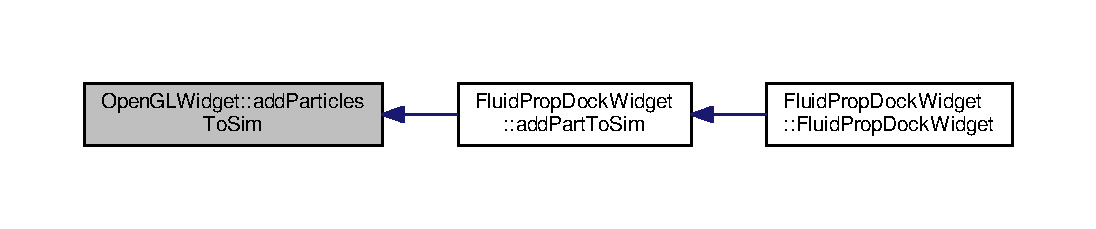
\includegraphics[width=350pt]{class_open_g_l_widget_adce23eb4fa8b5a1d1ac0403c911abb37_icgraph}
\end{center}
\end{figure}


\hypertarget{class_open_g_l_widget_a39018f8fc74ce591bfac884c277621e6}{\index{Open\-G\-L\-Widget@{Open\-G\-L\-Widget}!load\-Cube\-Map@{load\-Cube\-Map}}
\index{load\-Cube\-Map@{load\-Cube\-Map}!OpenGLWidget@{Open\-G\-L\-Widget}}
\subsubsection[{load\-Cube\-Map}]{\setlength{\rightskip}{0pt plus 5cm}void Open\-G\-L\-Widget\-::load\-Cube\-Map (
\begin{DoxyParamCaption}
\item[{Q\-String}]{\-\_\-loc}
\end{DoxyParamCaption}
)\hspace{0.3cm}{\ttfamily [slot]}}}\label{class_open_g_l_widget_a39018f8fc74ce591bfac884c277621e6}


slot to load cube maps to for our enironment map 

this function pressumes that all our cube map textures are in one texture 
\begin{DoxyParams}{Parameters}
{\em \-\_\-loc} & -\/ the location of our cube map texture \\
\hline
\end{DoxyParams}


Here is the caller graph for this function\-:\nopagebreak
\begin{figure}[H]
\begin{center}
\leavevmode
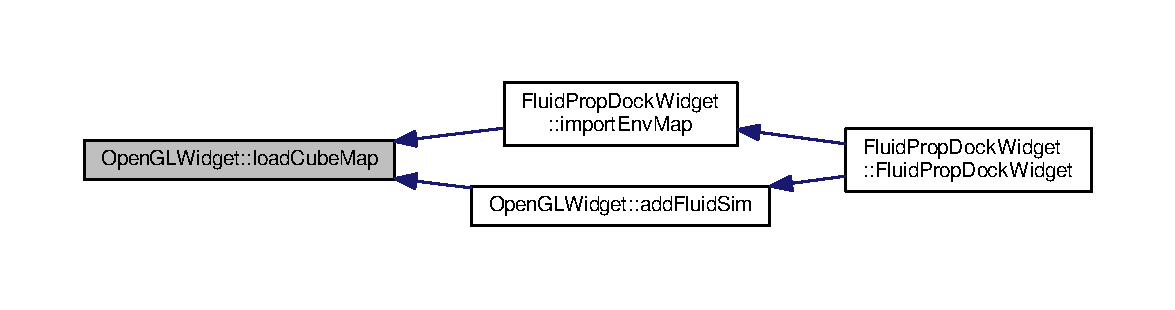
\includegraphics[width=350pt]{class_open_g_l_widget_a39018f8fc74ce591bfac884c277621e6_icgraph}
\end{center}
\end{figure}


\hypertarget{class_open_g_l_widget_a2d1d9bb18d20f1479cb86e832ab17fd2}{\index{Open\-G\-L\-Widget@{Open\-G\-L\-Widget}!play\-Toggle@{play\-Toggle}}
\index{play\-Toggle@{play\-Toggle}!OpenGLWidget@{Open\-G\-L\-Widget}}
\subsubsection[{play\-Toggle}]{\setlength{\rightskip}{0pt plus 5cm}void Open\-G\-L\-Widget\-::play\-Toggle (
\begin{DoxyParamCaption}
\item[{int}]{\-\_\-sim\-No = {\ttfamily 0}}
\end{DoxyParamCaption}
)\hspace{0.3cm}{\ttfamily [inline]}, {\ttfamily [slot]}}}\label{class_open_g_l_widget_a2d1d9bb18d20f1479cb86e832ab17fd2}


play/pause toggle slot 


\begin{DoxyParams}{Parameters}
{\em \-\_\-sim\-No} & -\/ which simulation we want to toggle play \\
\hline
\end{DoxyParams}


Here is the caller graph for this function\-:\nopagebreak
\begin{figure}[H]
\begin{center}
\leavevmode
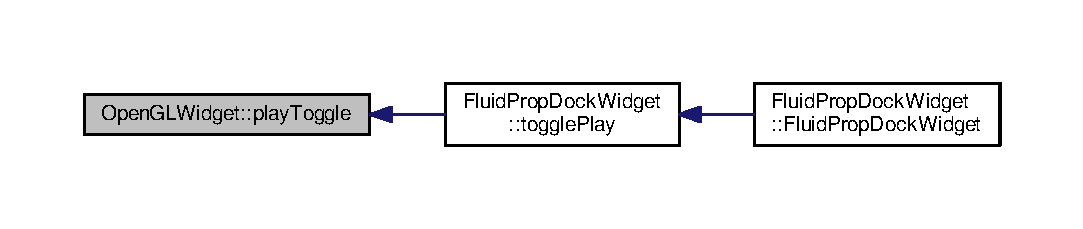
\includegraphics[width=350pt]{class_open_g_l_widget_a2d1d9bb18d20f1479cb86e832ab17fd2_icgraph}
\end{center}
\end{figure}


\hypertarget{class_open_g_l_widget_acc54210918549bd628db0080d576b483}{\index{Open\-G\-L\-Widget@{Open\-G\-L\-Widget}!reset\-Sim@{reset\-Sim}}
\index{reset\-Sim@{reset\-Sim}!OpenGLWidget@{Open\-G\-L\-Widget}}
\subsubsection[{reset\-Sim}]{\setlength{\rightskip}{0pt plus 5cm}void Open\-G\-L\-Widget\-::reset\-Sim (
\begin{DoxyParamCaption}
\item[{int}]{\-\_\-sim\-No}
\end{DoxyParamCaption}
)\hspace{0.3cm}{\ttfamily [inline]}, {\ttfamily [slot]}}}\label{class_open_g_l_widget_acc54210918549bd628db0080d576b483}


a slot to reset our simulation and remove all particles 

\-\_\-sim\-No -\/ simulation number to reset 

Here is the caller graph for this function\-:\nopagebreak
\begin{figure}[H]
\begin{center}
\leavevmode
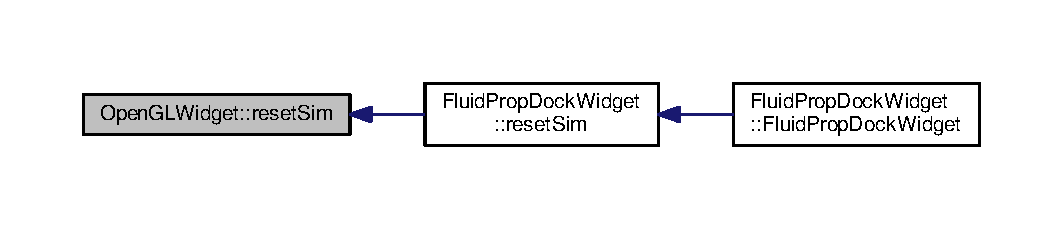
\includegraphics[width=350pt]{class_open_g_l_widget_acc54210918549bd628db0080d576b483_icgraph}
\end{center}
\end{figure}


\hypertarget{class_open_g_l_widget_a8e96b44ed40ec8a5fe726f427f01e6fe}{\index{Open\-G\-L\-Widget@{Open\-G\-L\-Widget}!set\-Blur\-Falloff@{set\-Blur\-Falloff}}
\index{set\-Blur\-Falloff@{set\-Blur\-Falloff}!OpenGLWidget@{Open\-G\-L\-Widget}}
\subsubsection[{set\-Blur\-Falloff}]{\setlength{\rightskip}{0pt plus 5cm}void Open\-G\-L\-Widget\-::set\-Blur\-Falloff (
\begin{DoxyParamCaption}
\item[{float}]{\-\_\-falloff, }
\item[{int}]{\-\_\-sim\-No = {\ttfamily 0}}
\end{DoxyParamCaption}
)\hspace{0.3cm}{\ttfamily [inline]}, {\ttfamily [slot]}}}\label{class_open_g_l_widget_a8e96b44ed40ec8a5fe726f427f01e6fe}


a slot to change our bilateral filter blur falloff 


\begin{DoxyParams}{Parameters}
{\em \-\_\-falloff} & -\/ bilateral blur falloff \\
\hline
{\em \-\_\-sim\-No} & -\/ which simulation we want to change the blur fall off in \\
\hline
\end{DoxyParams}


Here is the caller graph for this function\-:\nopagebreak
\begin{figure}[H]
\begin{center}
\leavevmode
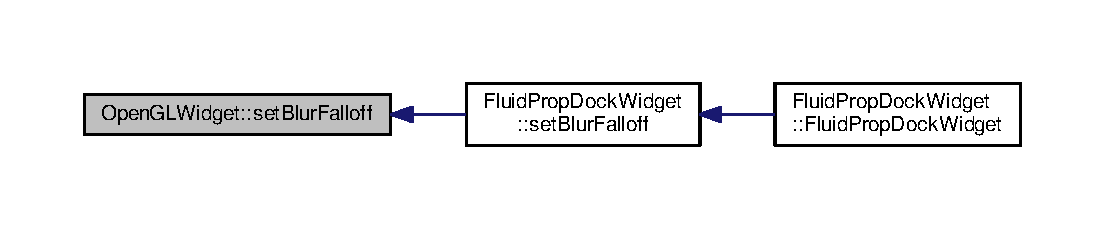
\includegraphics[width=350pt]{class_open_g_l_widget_a8e96b44ed40ec8a5fe726f427f01e6fe_icgraph}
\end{center}
\end{figure}


\hypertarget{class_open_g_l_widget_add467ba5217218564d08ffb638b2f190}{\index{Open\-G\-L\-Widget@{Open\-G\-L\-Widget}!set\-Blur\-Radius@{set\-Blur\-Radius}}
\index{set\-Blur\-Radius@{set\-Blur\-Radius}!OpenGLWidget@{Open\-G\-L\-Widget}}
\subsubsection[{set\-Blur\-Radius}]{\setlength{\rightskip}{0pt plus 5cm}void Open\-G\-L\-Widget\-::set\-Blur\-Radius (
\begin{DoxyParamCaption}
\item[{float}]{\-\_\-radius, }
\item[{int}]{\-\_\-sim\-No = {\ttfamily 0}}
\end{DoxyParamCaption}
)\hspace{0.3cm}{\ttfamily [inline]}, {\ttfamily [slot]}}}\label{class_open_g_l_widget_add467ba5217218564d08ffb638b2f190}


a slot to change our bilateral filter blur radius 


\begin{DoxyParams}{Parameters}
{\em \-\_\-radius} & -\/ bilateral blur radius \\
\hline
{\em \-\_\-sim\-No} & -\/ which simulation we want to change the blur radius in \\
\hline
\end{DoxyParams}


Here is the caller graph for this function\-:\nopagebreak
\begin{figure}[H]
\begin{center}
\leavevmode
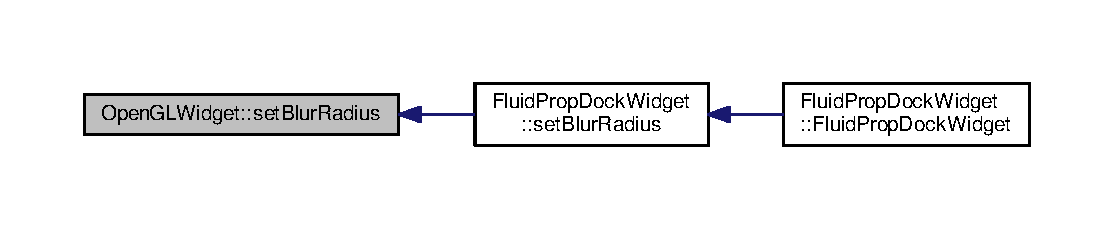
\includegraphics[width=350pt]{class_open_g_l_widget_add467ba5217218564d08ffb638b2f190_icgraph}
\end{center}
\end{figure}


\hypertarget{class_open_g_l_widget_a785cd8493ea4c1a24a19a16835de4577}{\index{Open\-G\-L\-Widget@{Open\-G\-L\-Widget}!set\-Density@{set\-Density}}
\index{set\-Density@{set\-Density}!OpenGLWidget@{Open\-G\-L\-Widget}}
\subsubsection[{set\-Density}]{\setlength{\rightskip}{0pt plus 5cm}void Open\-G\-L\-Widget\-::set\-Density (
\begin{DoxyParamCaption}
\item[{float}]{\-\_\-den, }
\item[{int}]{\-\_\-sim\-No = {\ttfamily 0}}
\end{DoxyParamCaption}
)\hspace{0.3cm}{\ttfamily [inline]}, {\ttfamily [slot]}}}\label{class_open_g_l_widget_a785cd8493ea4c1a24a19a16835de4577}


set density of our fluid slot 


\begin{DoxyParams}{Parameters}
{\em \-\_\-den} & -\/ desired rest density \\
\hline
{\em \-\_\-sim\-No} & -\/ which simulation we want to change \\
\hline
\end{DoxyParams}


Here is the caller graph for this function\-:\nopagebreak
\begin{figure}[H]
\begin{center}
\leavevmode
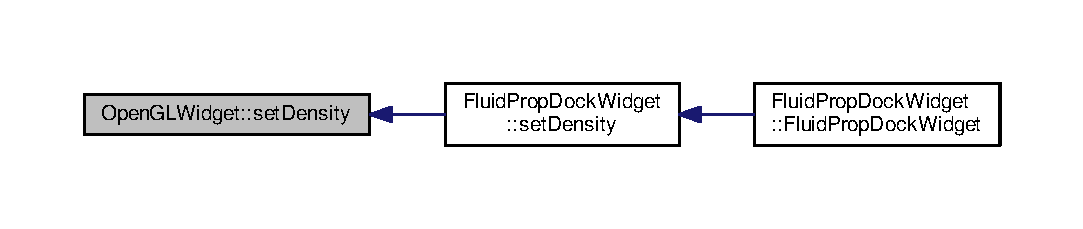
\includegraphics[width=350pt]{class_open_g_l_widget_a785cd8493ea4c1a24a19a16835de4577_icgraph}
\end{center}
\end{figure}


\hypertarget{class_open_g_l_widget_ac4dea29c4b53c1c4906dacd4aa35d975}{\index{Open\-G\-L\-Widget@{Open\-G\-L\-Widget}!set\-Display\-Hud@{set\-Display\-Hud}}
\index{set\-Display\-Hud@{set\-Display\-Hud}!OpenGLWidget@{Open\-G\-L\-Widget}}
\subsubsection[{set\-Display\-Hud}]{\setlength{\rightskip}{0pt plus 5cm}void Open\-G\-L\-Widget\-::set\-Display\-Hud (
\begin{DoxyParamCaption}
\item[{bool}]{\-\_\-display, }
\item[{int}]{\-\_\-sim\-No = {\ttfamily 0}}
\end{DoxyParamCaption}
)\hspace{0.3cm}{\ttfamily [inline]}, {\ttfamily [slot]}}}\label{class_open_g_l_widget_ac4dea29c4b53c1c4906dacd4aa35d975}


slot to toggle display of the hud of our simulatio 


\begin{DoxyParams}{Parameters}
{\em \-\_\-display} & -\/ bool to indicate if we want to display it or not \\
\hline
{\em \-\_\-sim\-No} & -\/ simulation we wish to display Hud \\
\hline
\end{DoxyParams}


Here is the caller graph for this function\-:\nopagebreak
\begin{figure}[H]
\begin{center}
\leavevmode
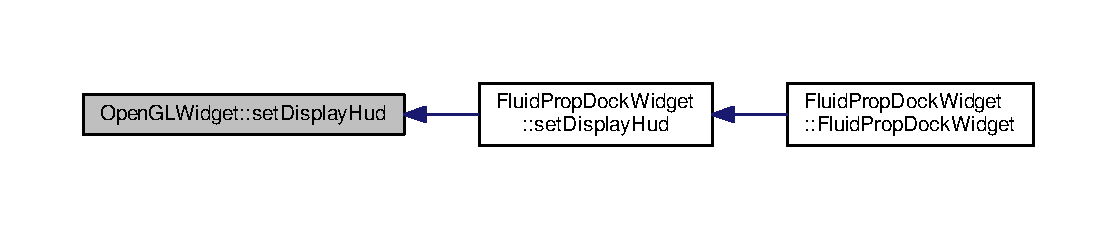
\includegraphics[width=350pt]{class_open_g_l_widget_ac4dea29c4b53c1c4906dacd4aa35d975_icgraph}
\end{center}
\end{figure}


\hypertarget{class_open_g_l_widget_a559ba717c412258c234ce5865c0b6976}{\index{Open\-G\-L\-Widget@{Open\-G\-L\-Widget}!set\-Fluid\-Color@{set\-Fluid\-Color}}
\index{set\-Fluid\-Color@{set\-Fluid\-Color}!OpenGLWidget@{Open\-G\-L\-Widget}}
\subsubsection[{set\-Fluid\-Color}]{\setlength{\rightskip}{0pt plus 5cm}void Open\-G\-L\-Widget\-::set\-Fluid\-Color (
\begin{DoxyParamCaption}
\item[{Q\-Color}]{\-\_\-col, }
\item[{int}]{\-\_\-sim\-No = {\ttfamily 0}}
\end{DoxyParamCaption}
)\hspace{0.3cm}{\ttfamily [inline]}, {\ttfamily [slot]}}}\label{class_open_g_l_widget_a559ba717c412258c234ce5865c0b6976}


set the color of our fluid slot 


\begin{DoxyParams}{Parameters}
{\em \-\_\-col} & -\/ desired color to set the fluid to \\
\hline
{\em \-\_\-sim\-No} & -\/ which simulation we want to change the color in \\
\hline
\end{DoxyParams}


Here is the caller graph for this function\-:\nopagebreak
\begin{figure}[H]
\begin{center}
\leavevmode
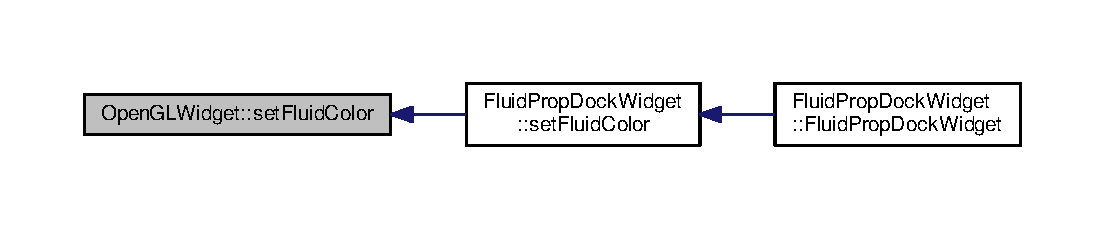
\includegraphics[width=350pt]{class_open_g_l_widget_a559ba717c412258c234ce5865c0b6976_icgraph}
\end{center}
\end{figure}


\hypertarget{class_open_g_l_widget_adc34d0b2bed5d7a7f2d5b92fa1b82889}{\index{Open\-G\-L\-Widget@{Open\-G\-L\-Widget}!set\-Fresnal\-Power@{set\-Fresnal\-Power}}
\index{set\-Fresnal\-Power@{set\-Fresnal\-Power}!OpenGLWidget@{Open\-G\-L\-Widget}}
\subsubsection[{set\-Fresnal\-Power}]{\setlength{\rightskip}{0pt plus 5cm}void Open\-G\-L\-Widget\-::set\-Fresnal\-Power (
\begin{DoxyParamCaption}
\item[{float}]{\-\_\-power, }
\item[{int}]{\-\_\-sim\-No = {\ttfamily 0}}
\end{DoxyParamCaption}
)\hspace{0.3cm}{\ttfamily [inline]}, {\ttfamily [slot]}}}\label{class_open_g_l_widget_adc34d0b2bed5d7a7f2d5b92fa1b82889}


a slot to set the fresnal power of our fluid 


\begin{DoxyParams}{Parameters}
{\em \-\_\-power} & -\/ desired fresnal power of our fluid \\
\hline
{\em \-\_\-sim\-No} & -\/ which simulation we want to change the fresnal power in \\
\hline
\end{DoxyParams}


Here is the caller graph for this function\-:\nopagebreak
\begin{figure}[H]
\begin{center}
\leavevmode
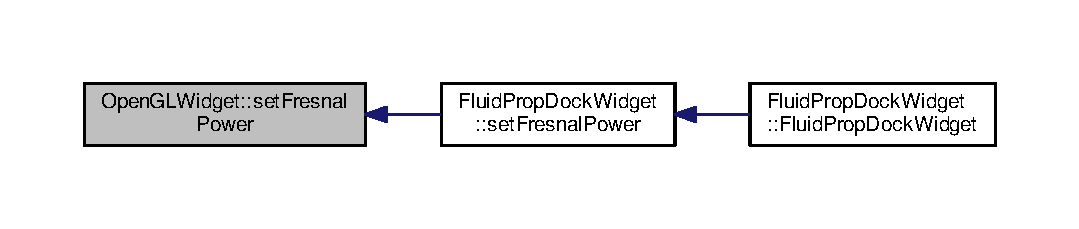
\includegraphics[width=350pt]{class_open_g_l_widget_adc34d0b2bed5d7a7f2d5b92fa1b82889_icgraph}
\end{center}
\end{figure}


\hypertarget{class_open_g_l_widget_a806e81697e0c6bf0992696ab948bc1c5}{\index{Open\-G\-L\-Widget@{Open\-G\-L\-Widget}!set\-Gas\-Const@{set\-Gas\-Const}}
\index{set\-Gas\-Const@{set\-Gas\-Const}!OpenGLWidget@{Open\-G\-L\-Widget}}
\subsubsection[{set\-Gas\-Const}]{\setlength{\rightskip}{0pt plus 5cm}void Open\-G\-L\-Widget\-::set\-Gas\-Const (
\begin{DoxyParamCaption}
\item[{double}]{\-\_\-gas\-Const, }
\item[{int}]{\-\_\-sim\-No = {\ttfamily 0}}
\end{DoxyParamCaption}
)\hspace{0.3cm}{\ttfamily [inline]}, {\ttfamily [slot]}}}\label{class_open_g_l_widget_a806e81697e0c6bf0992696ab948bc1c5}


set gas constant of our fluid slot 


\begin{DoxyParams}{Parameters}
{\em \-\_\-gas\-Const} & -\/ gas constant \\
\hline
{\em \-\_\-sim\-No} & -\/ which simulation we want to change \\
\hline
\end{DoxyParams}


Here is the caller graph for this function\-:\nopagebreak
\begin{figure}[H]
\begin{center}
\leavevmode
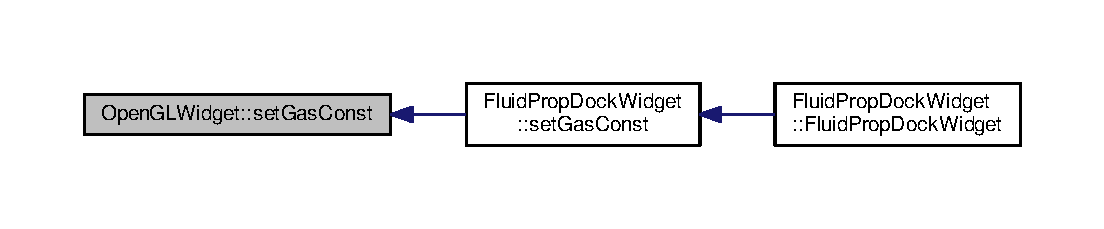
\includegraphics[width=350pt]{class_open_g_l_widget_a806e81697e0c6bf0992696ab948bc1c5_icgraph}
\end{center}
\end{figure}


\hypertarget{class_open_g_l_widget_a84585fd40a1fad03bbd118436f5fc477}{\index{Open\-G\-L\-Widget@{Open\-G\-L\-Widget}!set\-Mass@{set\-Mass}}
\index{set\-Mass@{set\-Mass}!OpenGLWidget@{Open\-G\-L\-Widget}}
\subsubsection[{set\-Mass}]{\setlength{\rightskip}{0pt plus 5cm}void Open\-G\-L\-Widget\-::set\-Mass (
\begin{DoxyParamCaption}
\item[{float}]{\-\_\-mass, }
\item[{int}]{\-\_\-sim\-No = {\ttfamily 0}}
\end{DoxyParamCaption}
)\hspace{0.3cm}{\ttfamily [inline]}, {\ttfamily [slot]}}}\label{class_open_g_l_widget_a84585fd40a1fad03bbd118436f5fc477}


set volume of our fluid slot 


\begin{DoxyParams}{Parameters}
{\em \-\_\-mass} & -\/ desired mass of particles \\
\hline
{\em \-\_\-sim\-No} & -\/ which simulation we want to change \\
\hline
\end{DoxyParams}


Here is the caller graph for this function\-:\nopagebreak
\begin{figure}[H]
\begin{center}
\leavevmode
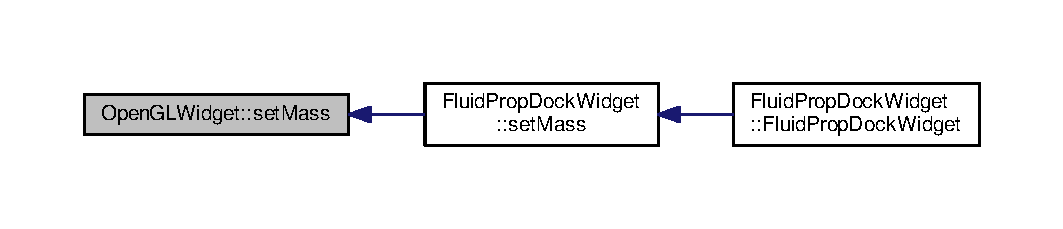
\includegraphics[width=350pt]{class_open_g_l_widget_a84585fd40a1fad03bbd118436f5fc477_icgraph}
\end{center}
\end{figure}


\hypertarget{class_open_g_l_widget_a3cdaf60ea4f98ee4782dec21b4810a41}{\index{Open\-G\-L\-Widget@{Open\-G\-L\-Widget}!set\-Particle\-Size@{set\-Particle\-Size}}
\index{set\-Particle\-Size@{set\-Particle\-Size}!OpenGLWidget@{Open\-G\-L\-Widget}}
\subsubsection[{set\-Particle\-Size}]{\setlength{\rightskip}{0pt plus 5cm}void Open\-G\-L\-Widget\-::set\-Particle\-Size (
\begin{DoxyParamCaption}
\item[{float}]{\-\_\-size, }
\item[{int}]{\-\_\-sim\-No = {\ttfamily 0}}
\end{DoxyParamCaption}
)\hspace{0.3cm}{\ttfamily [inline]}, {\ttfamily [slot]}}}\label{class_open_g_l_widget_a3cdaf60ea4f98ee4782dec21b4810a41}


a slot to change our particle size 


\begin{DoxyParams}{Parameters}
{\em \-\_\-size} & -\/ particle size \\
\hline
{\em \-\_\-sim\-No} & -\/ which simulation we want to change the particle size in \\
\hline
\end{DoxyParams}


Here is the caller graph for this function\-:\nopagebreak
\begin{figure}[H]
\begin{center}
\leavevmode
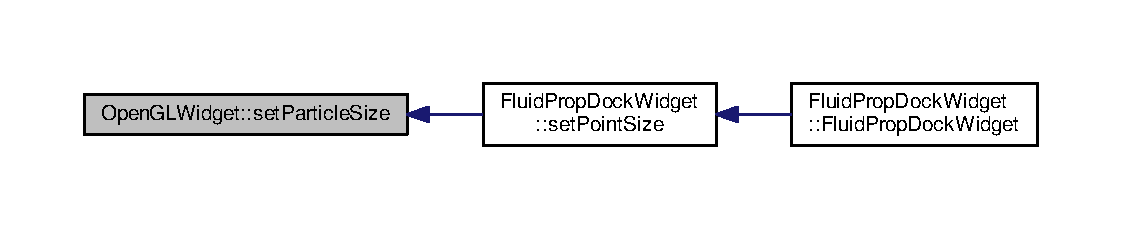
\includegraphics[width=350pt]{class_open_g_l_widget_a3cdaf60ea4f98ee4782dec21b4810a41_icgraph}
\end{center}
\end{figure}


\hypertarget{class_open_g_l_widget_aec967838bdff11519892bc05a5d930b0}{\index{Open\-G\-L\-Widget@{Open\-G\-L\-Widget}!set\-Particle\-Thickness@{set\-Particle\-Thickness}}
\index{set\-Particle\-Thickness@{set\-Particle\-Thickness}!OpenGLWidget@{Open\-G\-L\-Widget}}
\subsubsection[{set\-Particle\-Thickness}]{\setlength{\rightskip}{0pt plus 5cm}void Open\-G\-L\-Widget\-::set\-Particle\-Thickness (
\begin{DoxyParamCaption}
\item[{float}]{\-\_\-thickness, }
\item[{int}]{\-\_\-sim\-No = {\ttfamily 0}}
\end{DoxyParamCaption}
)\hspace{0.3cm}{\ttfamily [inline]}, {\ttfamily [slot]}}}\label{class_open_g_l_widget_aec967838bdff11519892bc05a5d930b0}


a slot to change our particle thickess 


\begin{DoxyParams}{Parameters}
{\em \-\_\-thickness} & -\/ particle thickness \\
\hline
{\em \-\_\-sim\-No} & -\/ which simulation we want to change the thickness in \\
\hline
\end{DoxyParams}


Here is the caller graph for this function\-:\nopagebreak
\begin{figure}[H]
\begin{center}
\leavevmode
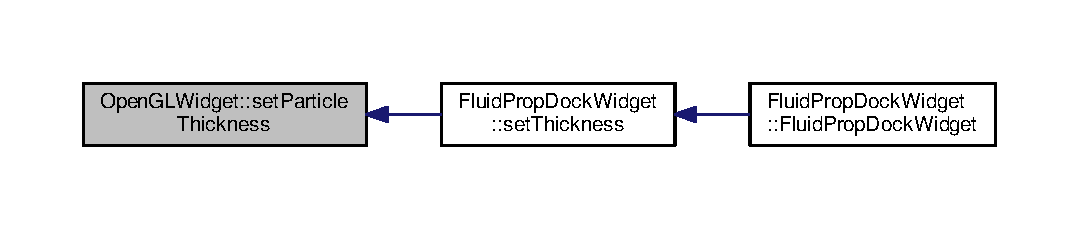
\includegraphics[width=350pt]{class_open_g_l_widget_aec967838bdff11519892bc05a5d930b0_icgraph}
\end{center}
\end{figure}


\hypertarget{class_open_g_l_widget_a3c415ea6ecc1ccf6df49b08df74bbd1a}{\index{Open\-G\-L\-Widget@{Open\-G\-L\-Widget}!set\-Playback\-Speed@{set\-Playback\-Speed}}
\index{set\-Playback\-Speed@{set\-Playback\-Speed}!OpenGLWidget@{Open\-G\-L\-Widget}}
\subsubsection[{set\-Playback\-Speed}]{\setlength{\rightskip}{0pt plus 5cm}void Open\-G\-L\-Widget\-::set\-Playback\-Speed (
\begin{DoxyParamCaption}
\item[{float}]{\-\_\-speed, }
\item[{int}]{\-\_\-sim\-No = {\ttfamily 0}}
\end{DoxyParamCaption}
)\hspace{0.3cm}{\ttfamily [inline]}, {\ttfamily [slot]}}}\label{class_open_g_l_widget_a3c415ea6ecc1ccf6df49b08df74bbd1a}


a slot to set the playback speed of our simulation 


\begin{DoxyParams}{Parameters}
{\em \-\_\-speed} & -\/ the speed of play back as a percentage 100.\-f is real time \\
\hline
{\em \-\_\-sim\-No} & -\/ which simulation we want to change the play back speed in \\
\hline
\end{DoxyParams}


Here is the caller graph for this function\-:\nopagebreak
\begin{figure}[H]
\begin{center}
\leavevmode
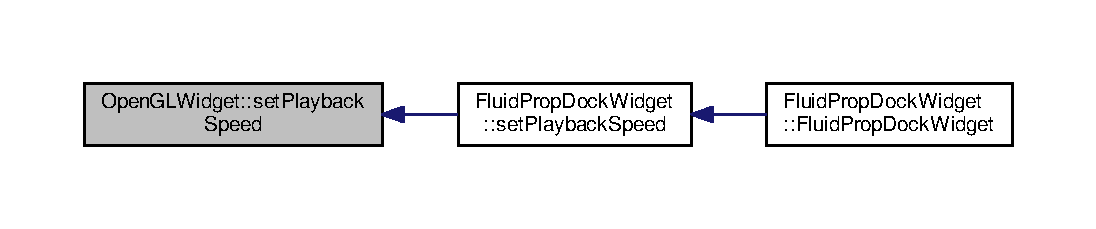
\includegraphics[width=350pt]{class_open_g_l_widget_a3c415ea6ecc1ccf6df49b08df74bbd1a_icgraph}
\end{center}
\end{figure}


\hypertarget{class_open_g_l_widget_a9ad49f35e3a76ec5ea58cedbe73afa34}{\index{Open\-G\-L\-Widget@{Open\-G\-L\-Widget}!set\-Rafraction\-Ratio@{set\-Rafraction\-Ratio}}
\index{set\-Rafraction\-Ratio@{set\-Rafraction\-Ratio}!OpenGLWidget@{Open\-G\-L\-Widget}}
\subsubsection[{set\-Rafraction\-Ratio}]{\setlength{\rightskip}{0pt plus 5cm}void Open\-G\-L\-Widget\-::set\-Rafraction\-Ratio (
\begin{DoxyParamCaption}
\item[{float}]{\-\_\-eta, }
\item[{int}]{\-\_\-sim\-No = {\ttfamily 0}}
\end{DoxyParamCaption}
)\hspace{0.3cm}{\ttfamily [inline]}, {\ttfamily [slot]}}}\label{class_open_g_l_widget_a9ad49f35e3a76ec5ea58cedbe73afa34}


a slot to set the refraction ratio of our fluid 


\begin{DoxyParams}{Parameters}
{\em \-\_\-eta} & -\/ desired refraction ratio \\
\hline
{\em \-\_\-sim\-No} & -\/ which simulation we want to change the rafraction ratio in \\
\hline
\end{DoxyParams}


Here is the caller graph for this function\-:\nopagebreak
\begin{figure}[H]
\begin{center}
\leavevmode
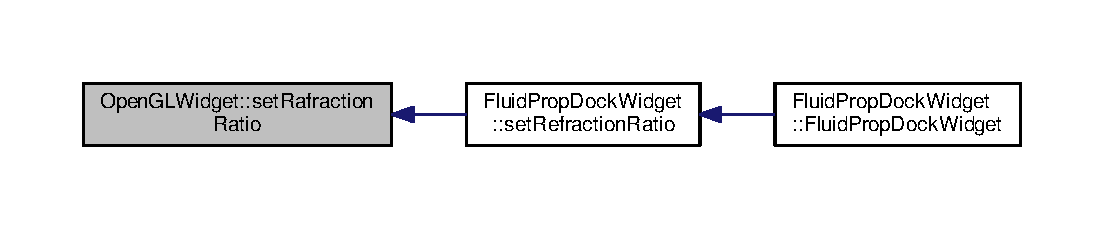
\includegraphics[width=350pt]{class_open_g_l_widget_a9ad49f35e3a76ec5ea58cedbe73afa34_icgraph}
\end{center}
\end{figure}


\hypertarget{class_open_g_l_widget_a6bc6106c82580697f386fdfd2fdb3a12}{\index{Open\-G\-L\-Widget@{Open\-G\-L\-Widget}!set\-Sim\-Position@{set\-Sim\-Position}}
\index{set\-Sim\-Position@{set\-Sim\-Position}!OpenGLWidget@{Open\-G\-L\-Widget}}
\subsubsection[{set\-Sim\-Position}]{\setlength{\rightskip}{0pt plus 5cm}void Open\-G\-L\-Widget\-::set\-Sim\-Position (
\begin{DoxyParamCaption}
\item[{float}]{\-\_\-x, }
\item[{float}]{\-\_\-y, }
\item[{float}]{\-\_\-z, }
\item[{int}]{\-\_\-sim\-No = {\ttfamily 0}}
\end{DoxyParamCaption}
)\hspace{0.3cm}{\ttfamily [inline]}, {\ttfamily [slot]}}}\label{class_open_g_l_widget_a6bc6106c82580697f386fdfd2fdb3a12}


slot to set sim position 


\begin{DoxyParams}{Parameters}
{\em \-\_\-x} & -\/ x position of our simulation \\
\hline
{\em \-\_\-y} & -\/ y position of our simulation \\
\hline
{\em \-\_\-z} & -\/ z position of our simualtion \\
\hline
{\em \-\_\-sim\-No} & -\/ simulation to set the position of \\
\hline
\end{DoxyParams}


Here is the caller graph for this function\-:\nopagebreak
\begin{figure}[H]
\begin{center}
\leavevmode
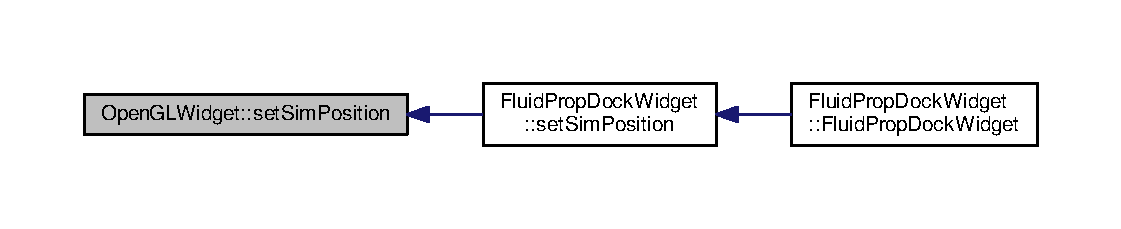
\includegraphics[width=350pt]{class_open_g_l_widget_a6bc6106c82580697f386fdfd2fdb3a12_icgraph}
\end{center}
\end{figure}


\hypertarget{class_open_g_l_widget_ac8a71d325740372032c0061d3bf1daa0}{\index{Open\-G\-L\-Widget@{Open\-G\-L\-Widget}!set\-Sim\-Time\-Step@{set\-Sim\-Time\-Step}}
\index{set\-Sim\-Time\-Step@{set\-Sim\-Time\-Step}!OpenGLWidget@{Open\-G\-L\-Widget}}
\subsubsection[{set\-Sim\-Time\-Step}]{\setlength{\rightskip}{0pt plus 5cm}void Open\-G\-L\-Widget\-::set\-Sim\-Time\-Step (
\begin{DoxyParamCaption}
\item[{float}]{\-\_\-time\-Step, }
\item[{int}]{\-\_\-sim\-No = {\ttfamily 0}}
\end{DoxyParamCaption}
)\hspace{0.3cm}{\ttfamily [inline]}, {\ttfamily [slot]}}}\label{class_open_g_l_widget_ac8a71d325740372032c0061d3bf1daa0}


a slot to set the time step of our simulation 


\begin{DoxyParams}{Parameters}
{\em \-\_\-time\-Step} & -\/ the time\-Step of our simulation \\
\hline
{\em \-\_\-sim\-No} & -\/ which simulation we want to change the play back speed in \\
\hline
\end{DoxyParams}


Here is the caller graph for this function\-:\nopagebreak
\begin{figure}[H]
\begin{center}
\leavevmode
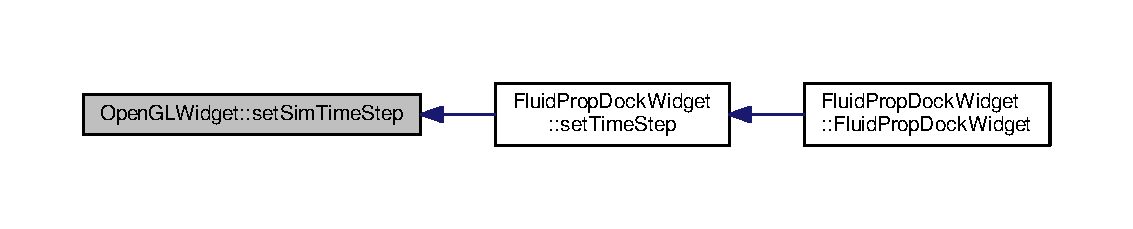
\includegraphics[width=350pt]{class_open_g_l_widget_ac8a71d325740372032c0061d3bf1daa0_icgraph}
\end{center}
\end{figure}


\hypertarget{class_open_g_l_widget_af0f0474b4ff16318e6cf2e7479b369c7}{\index{Open\-G\-L\-Widget@{Open\-G\-L\-Widget}!set\-Smoothing\-Length@{set\-Smoothing\-Length}}
\index{set\-Smoothing\-Length@{set\-Smoothing\-Length}!OpenGLWidget@{Open\-G\-L\-Widget}}
\subsubsection[{set\-Smoothing\-Length}]{\setlength{\rightskip}{0pt plus 5cm}void Open\-G\-L\-Widget\-::set\-Smoothing\-Length (
\begin{DoxyParamCaption}
\item[{float}]{\-\_\-len, }
\item[{int}]{\-\_\-sim\-No = {\ttfamily 0}}
\end{DoxyParamCaption}
)\hspace{0.3cm}{\ttfamily [inline]}, {\ttfamily [slot]}}}\label{class_open_g_l_widget_af0f0474b4ff16318e6cf2e7479b369c7}


set smoothing length of our fluid slot 


\begin{DoxyParams}{Parameters}
{\em \-\_\-len} & -\/ smoothing length \\
\hline
{\em \-\_\-sim\-No} & -\/ which simulation we want to change our smoothing length in \\
\hline
\end{DoxyParams}


Here is the caller graph for this function\-:\nopagebreak
\begin{figure}[H]
\begin{center}
\leavevmode
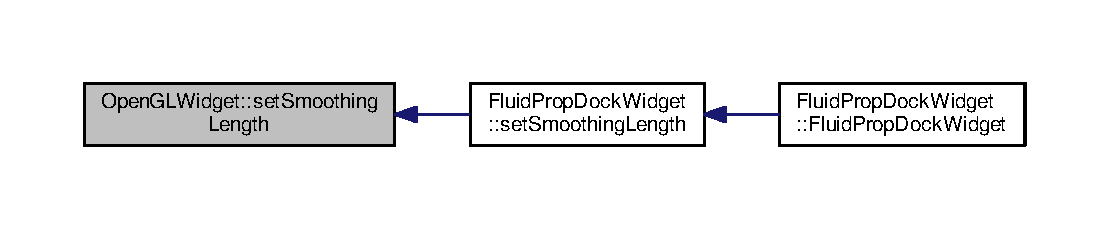
\includegraphics[width=350pt]{class_open_g_l_widget_af0f0474b4ff16318e6cf2e7479b369c7_icgraph}
\end{center}
\end{figure}


\hypertarget{class_open_g_l_widget_ac4d67ea702f268f7d072e94a569cb5f0}{\index{Open\-G\-L\-Widget@{Open\-G\-L\-Widget}!set\-Spawn\-Box\-Position@{set\-Spawn\-Box\-Position}}
\index{set\-Spawn\-Box\-Position@{set\-Spawn\-Box\-Position}!OpenGLWidget@{Open\-G\-L\-Widget}}
\subsubsection[{set\-Spawn\-Box\-Position}]{\setlength{\rightskip}{0pt plus 5cm}void Open\-G\-L\-Widget\-::set\-Spawn\-Box\-Position (
\begin{DoxyParamCaption}
\item[{float}]{\-\_\-x, }
\item[{float}]{\-\_\-y, }
\item[{float}]{\-\_\-z, }
\item[{int}]{\-\_\-sim\-No = {\ttfamily 0}}
\end{DoxyParamCaption}
)\hspace{0.3cm}{\ttfamily [inline]}, {\ttfamily [slot]}}}\label{class_open_g_l_widget_ac4d67ea702f268f7d072e94a569cb5f0}


a slot to set the spawn box position in our simulation 


\begin{DoxyParams}{Parameters}
{\em \-\_\-x} & -\/ x position of spawn box location \\
\hline
{\em \-\_\-y} & -\/ y position of spawn box location \\
\hline
{\em \-\_\-z} & -\/ z position of spawn box location \\
\hline
{\em \-\_\-sim\-No} & -\/ simulation number to set the spawn box location \\
\hline
\end{DoxyParams}


Here is the caller graph for this function\-:\nopagebreak
\begin{figure}[H]
\begin{center}
\leavevmode
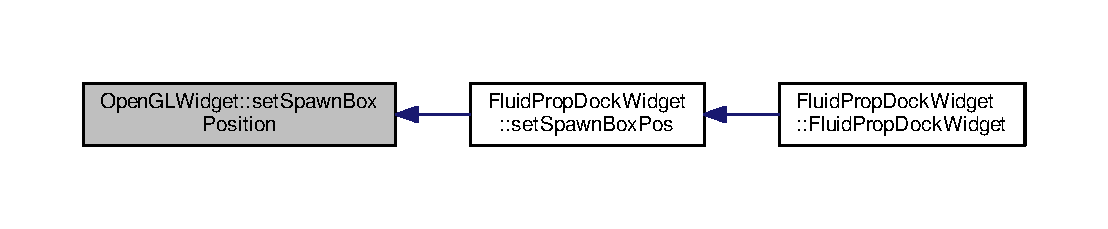
\includegraphics[width=350pt]{class_open_g_l_widget_ac4d67ea702f268f7d072e94a569cb5f0_icgraph}
\end{center}
\end{figure}


\hypertarget{class_open_g_l_widget_a60e5e6f2845384c3faeaa11c0fb800b4}{\index{Open\-G\-L\-Widget@{Open\-G\-L\-Widget}!set\-Spawn\-Box\-Size@{set\-Spawn\-Box\-Size}}
\index{set\-Spawn\-Box\-Size@{set\-Spawn\-Box\-Size}!OpenGLWidget@{Open\-G\-L\-Widget}}
\subsubsection[{set\-Spawn\-Box\-Size}]{\setlength{\rightskip}{0pt plus 5cm}void Open\-G\-L\-Widget\-::set\-Spawn\-Box\-Size (
\begin{DoxyParamCaption}
\item[{float}]{\-\_\-size, }
\item[{int}]{\-\_\-sim\-No = {\ttfamily 0}}
\end{DoxyParamCaption}
)\hspace{0.3cm}{\ttfamily [inline]}, {\ttfamily [slot]}}}\label{class_open_g_l_widget_a60e5e6f2845384c3faeaa11c0fb800b4}


a slot to set the spawn box size in our simulation 


\begin{DoxyParams}{Parameters}
{\em \-\_\-size} & -\/ desired spawn box size \\
\hline
{\em \-\_\-sim\-No} & -\/ simulation number to set the spawn box size \\
\hline
\end{DoxyParams}


Here is the caller graph for this function\-:\nopagebreak
\begin{figure}[H]
\begin{center}
\leavevmode
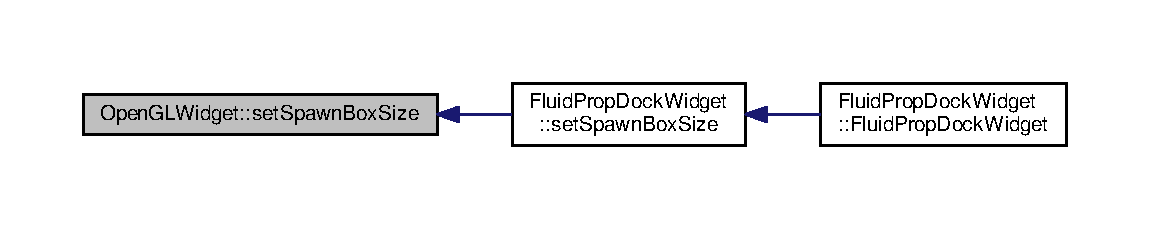
\includegraphics[width=350pt]{class_open_g_l_widget_a60e5e6f2845384c3faeaa11c0fb800b4_icgraph}
\end{center}
\end{figure}


\hypertarget{class_open_g_l_widget_a9ca3397753dcfbc56ada94d1e91000ed}{\index{Open\-G\-L\-Widget@{Open\-G\-L\-Widget}!set\-Vel\-Correction@{set\-Vel\-Correction}}
\index{set\-Vel\-Correction@{set\-Vel\-Correction}!OpenGLWidget@{Open\-G\-L\-Widget}}
\subsubsection[{set\-Vel\-Correction}]{\setlength{\rightskip}{0pt plus 5cm}void Open\-G\-L\-Widget\-::set\-Vel\-Correction (
\begin{DoxyParamCaption}
\item[{float}]{\-\_\-val, }
\item[{int}]{\-\_\-sim\-No = {\ttfamily 0}}
\end{DoxyParamCaption}
)\hspace{0.3cm}{\ttfamily [inline]}, {\ttfamily [slot]}}}\label{class_open_g_l_widget_a9ca3397753dcfbc56ada94d1e91000ed}


slot to set the velocity correction of our simulation 


\begin{DoxyParams}{Parameters}
{\em \-\_\-val} & -\/ value of velocity correction \\
\hline
{\em \-\_\-sim\-No} & -\/ simulation to set velocity correction in \\
\hline
\end{DoxyParams}


Here is the caller graph for this function\-:\nopagebreak
\begin{figure}[H]
\begin{center}
\leavevmode
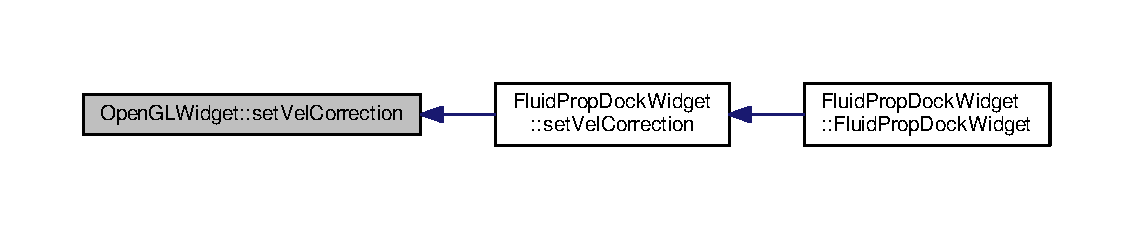
\includegraphics[width=350pt]{class_open_g_l_widget_a9ca3397753dcfbc56ada94d1e91000ed_icgraph}
\end{center}
\end{figure}


\hypertarget{class_open_g_l_widget_aad4c9ceaedc57507d3e9504d15dd8f4a}{\index{Open\-G\-L\-Widget@{Open\-G\-L\-Widget}!set\-Visc\-Coef@{set\-Visc\-Coef}}
\index{set\-Visc\-Coef@{set\-Visc\-Coef}!OpenGLWidget@{Open\-G\-L\-Widget}}
\subsubsection[{set\-Visc\-Coef}]{\setlength{\rightskip}{0pt plus 5cm}void Open\-G\-L\-Widget\-::set\-Visc\-Coef (
\begin{DoxyParamCaption}
\item[{float}]{\-\_\-visc, }
\item[{int}]{\-\_\-sim\-No = {\ttfamily 0}}
\end{DoxyParamCaption}
)\hspace{0.3cm}{\ttfamily [inline]}, {\ttfamily [slot]}}}\label{class_open_g_l_widget_aad4c9ceaedc57507d3e9504d15dd8f4a}


set viscoty coeficient of our fluid slot 


\begin{DoxyParams}{Parameters}
{\em \-\_\-visc} & -\/ viscosity coeficient \\
\hline
{\em \-\_\-sim\-No} & -\/ which simulation we want to change \\
\hline
\end{DoxyParams}


Here is the caller graph for this function\-:\nopagebreak
\begin{figure}[H]
\begin{center}
\leavevmode
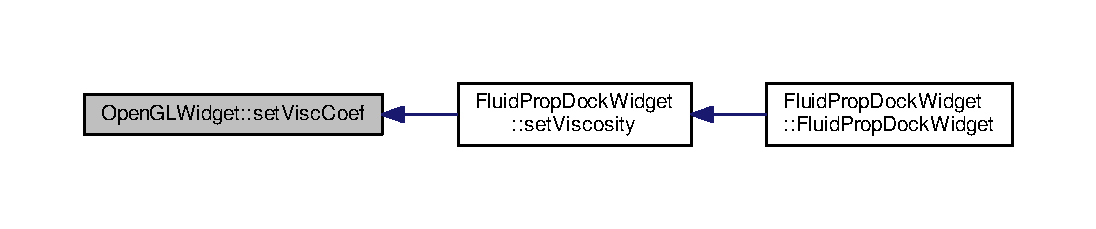
\includegraphics[width=350pt]{class_open_g_l_widget_aad4c9ceaedc57507d3e9504d15dd8f4a_icgraph}
\end{center}
\end{figure}


\hypertarget{class_open_g_l_widget_a0682546d360b7ce9ae1dce31a090cfca}{\index{Open\-G\-L\-Widget@{Open\-G\-L\-Widget}!wheel\-Event@{wheel\-Event}}
\index{wheel\-Event@{wheel\-Event}!OpenGLWidget@{Open\-G\-L\-Widget}}
\subsubsection[{wheel\-Event}]{\setlength{\rightskip}{0pt plus 5cm}void Open\-G\-L\-Widget\-::wheel\-Event (
\begin{DoxyParamCaption}
\item[{Q\-Wheel\-Event $\ast$}]{\-\_\-event}
\end{DoxyParamCaption}
)}}\label{class_open_g_l_widget_a0682546d360b7ce9ae1dce31a090cfca}


this method is called everytime the mouse wheel is moved inherited from Q\-Object and overridden here. 


\begin{DoxyParams}{Parameters}
{\em \-\_\-event} & the Qt Event structure \\
\hline
\end{DoxyParams}


The documentation for this class was generated from the following files\-:\begin{DoxyCompactItemize}
\item 
/home/dexternation/\-A\-G\-S\-D\-T\-Fluid\-Sim/include/\hyperlink{_open_g_l_widget_8h}{Open\-G\-L\-Widget.\-h}\item 
/home/dexternation/\-A\-G\-S\-D\-T\-Fluid\-Sim/src/Open\-G\-L\-Widget.\-cpp\end{DoxyCompactItemize}

\hypertarget{structqt__meta__stringdata___fluid_prop_dock_widget__t}{\section{qt\-\_\-meta\-\_\-stringdata\-\_\-\-Fluid\-Prop\-Dock\-Widget\-\_\-t Struct Reference}
\label{structqt__meta__stringdata___fluid_prop_dock_widget__t}\index{qt\-\_\-meta\-\_\-stringdata\-\_\-\-Fluid\-Prop\-Dock\-Widget\-\_\-t@{qt\-\_\-meta\-\_\-stringdata\-\_\-\-Fluid\-Prop\-Dock\-Widget\-\_\-t}}
}


Collaboration diagram for qt\-\_\-meta\-\_\-stringdata\-\_\-\-Fluid\-Prop\-Dock\-Widget\-\_\-t\-:\nopagebreak
\begin{figure}[H]
\begin{center}
\leavevmode
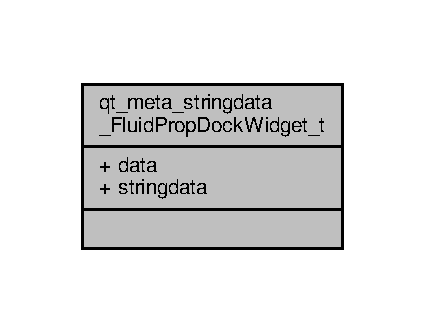
\includegraphics[width=204pt]{structqt__meta__stringdata___fluid_prop_dock_widget__t__coll__graph}
\end{center}
\end{figure}
\subsection*{Public Attributes}
\begin{DoxyCompactItemize}
\item 
\hypertarget{structqt__meta__stringdata___fluid_prop_dock_widget__t_a4ec27da0a498540f17a8b4012ba7010a}{Q\-Byte\-Array\-Data {\bfseries data} \mbox{[}41\mbox{]}}\label{structqt__meta__stringdata___fluid_prop_dock_widget__t_a4ec27da0a498540f17a8b4012ba7010a}

\item 
\hypertarget{structqt__meta__stringdata___fluid_prop_dock_widget__t_a853bb9fbb11a9682d7c74ce25980bf6c}{char {\bfseries stringdata} \mbox{[}453\mbox{]}}\label{structqt__meta__stringdata___fluid_prop_dock_widget__t_a853bb9fbb11a9682d7c74ce25980bf6c}

\end{DoxyCompactItemize}


The documentation for this struct was generated from the following file\-:\begin{DoxyCompactItemize}
\item 
/home/dexternation/\-A\-G\-S\-D\-T\-Fluid\-Sim/moc/moc\-\_\-\-Fluid\-Prop\-Dock\-Widget.\-cpp\end{DoxyCompactItemize}

\hypertarget{structqt__meta__stringdata___main_window__t}{\section{qt\-\_\-meta\-\_\-stringdata\-\_\-\-Main\-Window\-\_\-t Struct Reference}
\label{structqt__meta__stringdata___main_window__t}\index{qt\-\_\-meta\-\_\-stringdata\-\_\-\-Main\-Window\-\_\-t@{qt\-\_\-meta\-\_\-stringdata\-\_\-\-Main\-Window\-\_\-t}}
}


Collaboration diagram for qt\-\_\-meta\-\_\-stringdata\-\_\-\-Main\-Window\-\_\-t\-:
\subsection*{Public Attributes}
\begin{DoxyCompactItemize}
\item 
\hypertarget{structqt__meta__stringdata___main_window__t_a0a55531510dd06148b7b0f445e2b6c59}{Q\-Byte\-Array\-Data {\bfseries data} \mbox{[}3\mbox{]}}\label{structqt__meta__stringdata___main_window__t_a0a55531510dd06148b7b0f445e2b6c59}

\item 
\hypertarget{structqt__meta__stringdata___main_window__t_a22301b390de7f6e6864deb255884e5f9}{char {\bfseries stringdata} \mbox{[}21\mbox{]}}\label{structqt__meta__stringdata___main_window__t_a22301b390de7f6e6864deb255884e5f9}

\end{DoxyCompactItemize}


The documentation for this struct was generated from the following file\-:\begin{DoxyCompactItemize}
\item 
moc/moc\-\_\-mainwindow.\-cpp\end{DoxyCompactItemize}

\hypertarget{structqt__meta__stringdata___open_g_l_widget__t}{\section{qt\-\_\-meta\-\_\-stringdata\-\_\-\-Open\-G\-L\-Widget\-\_\-t Struct Reference}
\label{structqt__meta__stringdata___open_g_l_widget__t}\index{qt\-\_\-meta\-\_\-stringdata\-\_\-\-Open\-G\-L\-Widget\-\_\-t@{qt\-\_\-meta\-\_\-stringdata\-\_\-\-Open\-G\-L\-Widget\-\_\-t}}
}


Collaboration diagram for qt\-\_\-meta\-\_\-stringdata\-\_\-\-Open\-G\-L\-Widget\-\_\-t\-:\nopagebreak
\begin{figure}[H]
\begin{center}
\leavevmode
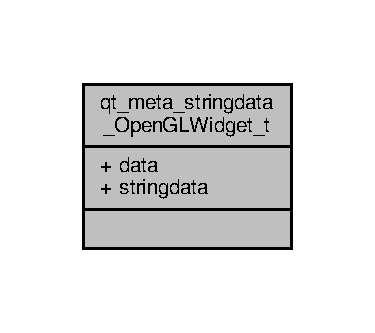
\includegraphics[width=180pt]{structqt__meta__stringdata___open_g_l_widget__t__coll__graph}
\end{center}
\end{figure}
\subsection*{Public Attributes}
\begin{DoxyCompactItemize}
\item 
\hypertarget{structqt__meta__stringdata___open_g_l_widget__t_ad12a546ae59866732c758206e9e72938}{Q\-Byte\-Array\-Data {\bfseries data} \mbox{[}48\mbox{]}}\label{structqt__meta__stringdata___open_g_l_widget__t_ad12a546ae59866732c758206e9e72938}

\item 
\hypertarget{structqt__meta__stringdata___open_g_l_widget__t_a356daa95022344d6aa7de96775220623}{char {\bfseries stringdata} \mbox{[}517\mbox{]}}\label{structqt__meta__stringdata___open_g_l_widget__t_a356daa95022344d6aa7de96775220623}

\end{DoxyCompactItemize}


The documentation for this struct was generated from the following file\-:\begin{DoxyCompactItemize}
\item 
/home/dexternation/\-A\-G\-S\-D\-T\-Fluid\-Sim/moc/moc\-\_\-\-Open\-G\-L\-Widget.\-cpp\end{DoxyCompactItemize}

\hypertarget{class_render_buffer}{\section{Render\-Buffer Class Reference}
\label{class_render_buffer}\index{Render\-Buffer@{Render\-Buffer}}
}


Class for creating render buffers.  




{\ttfamily \#include $<$Render\-Buffer.\-h$>$}



Inheritance diagram for Render\-Buffer\-:


Collaboration diagram for Render\-Buffer\-:
\subsection*{Public Member Functions}
\begin{DoxyCompactItemize}
\item 
\hypertarget{class_render_buffer_ac3494e7208c1b9fee4e0ff61b24d38ee}{\hyperlink{class_render_buffer_ac3494e7208c1b9fee4e0ff61b24d38ee}{Render\-Buffer} (G\-Lenum \-\_\-internalformat, G\-Lenum \-\_\-attachment, G\-Lsizei \-\_\-width, G\-Lsizei \-\_\-height)}\label{class_render_buffer_ac3494e7208c1b9fee4e0ff61b24d38ee}

\begin{DoxyCompactList}\small\item\em default constructor creates our render buffer \end{DoxyCompactList}\item 
\hypertarget{class_render_buffer_a19e7ab6e01523fffea6d5415510889d6}{\hyperlink{class_render_buffer_a19e7ab6e01523fffea6d5415510889d6}{$\sim$\-Render\-Buffer} ()}\label{class_render_buffer_a19e7ab6e01523fffea6d5415510889d6}

\begin{DoxyCompactList}\small\item\em default destructor deletes render buffer \end{DoxyCompactList}\item 
\hypertarget{class_render_buffer_ae0ae7cf1d85a6a4bee741a0132b2b8ab}{void \hyperlink{class_render_buffer_ae0ae7cf1d85a6a4bee741a0132b2b8ab}{bind} ()}\label{class_render_buffer_ae0ae7cf1d85a6a4bee741a0132b2b8ab}

\begin{DoxyCompactList}\small\item\em binds our render buffer \end{DoxyCompactList}\item 
\hypertarget{class_render_buffer_aacb6894f0d626da9e35c383674be7f86}{void \hyperlink{class_render_buffer_aacb6894f0d626da9e35c383674be7f86}{unbind} ()}\label{class_render_buffer_aacb6894f0d626da9e35c383674be7f86}

\begin{DoxyCompactList}\small\item\em unbinds our render buffer \end{DoxyCompactList}\item 
void \hyperlink{class_render_buffer_a7dfe2482e11ec51c8ebd687d9ff0a045}{resize} (G\-Lsizei \-\_\-width, G\-Lsizei \-\_\-height)
\begin{DoxyCompactList}\small\item\em reizes our render buffer \end{DoxyCompactList}\end{DoxyCompactItemize}
\subsection*{Private Attributes}
\begin{DoxyCompactItemize}
\item 
\hypertarget{class_render_buffer_a897cca2ee9529f82447fee545354135f}{G\-Lsizei \hyperlink{class_render_buffer_a897cca2ee9529f82447fee545354135f}{m\-\_\-width}}\label{class_render_buffer_a897cca2ee9529f82447fee545354135f}

\begin{DoxyCompactList}\small\item\em width of our render buffer \end{DoxyCompactList}\item 
\hypertarget{class_render_buffer_a747f5fc28706771541141a6a581031dc}{G\-Lsizei \hyperlink{class_render_buffer_a747f5fc28706771541141a6a581031dc}{m\-\_\-height}}\label{class_render_buffer_a747f5fc28706771541141a6a581031dc}

\begin{DoxyCompactList}\small\item\em height of our render buffer \end{DoxyCompactList}\item 
\hypertarget{class_render_buffer_a07f819fc22c10d7aea614d9aef443c72}{G\-Lenum \hyperlink{class_render_buffer_a07f819fc22c10d7aea614d9aef443c72}{m\-\_\-internal\-Format}}\label{class_render_buffer_a07f819fc22c10d7aea614d9aef443c72}

\begin{DoxyCompactList}\small\item\em internal format of our render target \end{DoxyCompactList}\end{DoxyCompactItemize}
\subsection*{Additional Inherited Members}


\subsection{Detailed Description}
Class for creating render buffers. 

\begin{DoxyAuthor}{Author}
Declan Russell 
\end{DoxyAuthor}
\begin{DoxyDate}{Date}
28/04/2015 
\end{DoxyDate}
\begin{DoxyVersion}{Version}
1.\-0 
\end{DoxyVersion}


\subsection{Member Function Documentation}
\hypertarget{class_render_buffer_a7dfe2482e11ec51c8ebd687d9ff0a045}{\index{Render\-Buffer@{Render\-Buffer}!resize@{resize}}
\index{resize@{resize}!RenderBuffer@{Render\-Buffer}}
\subsubsection[{resize}]{\setlength{\rightskip}{0pt plus 5cm}void Render\-Buffer\-::resize (
\begin{DoxyParamCaption}
\item[{G\-Lsizei}]{\-\_\-width, }
\item[{G\-Lsizei}]{\-\_\-height}
\end{DoxyParamCaption}
)}}\label{class_render_buffer_a7dfe2482e11ec51c8ebd687d9ff0a045}


reizes our render buffer 


\begin{DoxyParams}{Parameters}
{\em \-\_\-width} & -\/ deisred width of render buffer \\
\hline
{\em \-\_\-height} & -\/ desired height of render buffer \\
\hline
\end{DoxyParams}


Here is the call graph for this function\-:




The documentation for this class was generated from the following files\-:\begin{DoxyCompactItemize}
\item 
include/\hyperlink{_render_buffer_8h}{Render\-Buffer.\-h}\item 
src/Render\-Buffer.\-cpp\end{DoxyCompactItemize}

\hypertarget{class_render_target_lib}{\section{Render\-Target\-Lib Class Reference}
\label{class_render_target_lib}\index{Render\-Target\-Lib@{Render\-Target\-Lib}}
}


Singleton class for creating and storing render targets in a library.  




{\ttfamily \#include $<$Render\-Target\-Lib.\-h$>$}



Collaboration diagram for Render\-Target\-Lib\-:
\subsection*{Public Member Functions}
\begin{DoxyCompactItemize}
\item 
\hyperlink{class_render_buffer}{Render\-Buffer} $\ast$ \hyperlink{class_render_target_lib_a0ff27ec9ae3c085a2bce4e05c180e0e3}{add\-Render\-Buffer} (std\-::string \-\_\-name, G\-Lenum \-\_\-internalformat, G\-Lenum \-\_\-attachment, G\-Lsizei \-\_\-width, G\-Lsizei \-\_\-height)
\begin{DoxyCompactList}\small\item\em add a render buffer to our library \end{DoxyCompactList}\item 
\hypertarget{class_render_target_lib_ac5971bca0f97cedf1e7c16d8d1233fdc}{\hyperlink{class_frame_buffer}{Frame\-Buffer} $\ast$ \hyperlink{class_render_target_lib_ac5971bca0f97cedf1e7c16d8d1233fdc}{add\-Frame\-Buffer} (std\-::string \-\_\-name)}\label{class_render_target_lib_ac5971bca0f97cedf1e7c16d8d1233fdc}

\begin{DoxyCompactList}\small\item\em add a frame buffer to our library \end{DoxyCompactList}\item 
\hypertarget{class_render_target_lib_a30afc5063831926612da80726dea0f04}{\hyperlink{class_frame_buffer}{Frame\-Buffer} $\ast$ \hyperlink{class_render_target_lib_a30afc5063831926612da80726dea0f04}{get\-Frame\-Buffer} (const std\-::string \&\-\_\-name)}\label{class_render_target_lib_a30afc5063831926612da80726dea0f04}

\begin{DoxyCompactList}\small\item\em gets a frame buffer from our library \end{DoxyCompactList}\item 
\hypertarget{class_render_target_lib_a9695e1a845c84e76c10bec26460b0e8b}{\hyperlink{class_frame_buffer}{Frame\-Buffer} $\ast$ \hyperlink{class_render_target_lib_a9695e1a845c84e76c10bec26460b0e8b}{get\-Frame\-Buffer} (const char $\ast$\-\_\-name)}\label{class_render_target_lib_a9695e1a845c84e76c10bec26460b0e8b}

\begin{DoxyCompactList}\small\item\em gets a frame buffer from our library \end{DoxyCompactList}\item 
\hypertarget{class_render_target_lib_acf1fa30e68dc74deca512b0c77786d0a}{\hyperlink{class_render_buffer}{Render\-Buffer} $\ast$ \hyperlink{class_render_target_lib_acf1fa30e68dc74deca512b0c77786d0a}{get\-Render\-Buffer} (const std\-::string \&\-\_\-name)}\label{class_render_target_lib_acf1fa30e68dc74deca512b0c77786d0a}

\begin{DoxyCompactList}\small\item\em gets a render buffer from our library \end{DoxyCompactList}\item 
\hypertarget{class_render_target_lib_aeda9a8138eef8e87558431809933074b}{\hyperlink{class_render_buffer}{Render\-Buffer} $\ast$ \hyperlink{class_render_target_lib_aeda9a8138eef8e87558431809933074b}{get\-Render\-Buffer} (const char $\ast$\-\_\-name)}\label{class_render_target_lib_aeda9a8138eef8e87558431809933074b}

\begin{DoxyCompactList}\small\item\em gets a render buffer from our library \end{DoxyCompactList}\item 
\hypertarget{class_render_target_lib_a71b6707d4e877c56cf167bee8995ff6a}{void \hyperlink{class_render_target_lib_a71b6707d4e877c56cf167bee8995ff6a}{destroy} ()}\label{class_render_target_lib_a71b6707d4e877c56cf167bee8995ff6a}

\begin{DoxyCompactList}\small\item\em Deletes our library. \end{DoxyCompactList}\end{DoxyCompactItemize}
\subsection*{Static Public Member Functions}
\begin{DoxyCompactItemize}
\item 
\hypertarget{class_render_target_lib_a99e969c4379b3c037b3152ae4603e436}{static \hyperlink{class_render_target_lib}{Render\-Target\-Lib} $\ast$ \hyperlink{class_render_target_lib_a99e969c4379b3c037b3152ae4603e436}{get\-Instance} ()}\label{class_render_target_lib_a99e969c4379b3c037b3152ae4603e436}

\begin{DoxyCompactList}\small\item\em returns an instance of our render target library \end{DoxyCompactList}\end{DoxyCompactItemize}
\subsection*{Private Member Functions}
\begin{DoxyCompactItemize}
\item 
\hypertarget{class_render_target_lib_a0ae1e327dc608b42223cf41de7363110}{\hyperlink{class_render_target_lib_a0ae1e327dc608b42223cf41de7363110}{$\sim$\-Render\-Target\-Lib} ()}\label{class_render_target_lib_a0ae1e327dc608b42223cf41de7363110}

\begin{DoxyCompactList}\small\item\em our destructor. Removes all render targets from library \end{DoxyCompactList}\item 
\hypertarget{class_render_target_lib_aca1daab0d875c1e27e95d290851b1870}{\hyperlink{class_render_target_lib_aca1daab0d875c1e27e95d290851b1870}{Render\-Target\-Lib} ()}\label{class_render_target_lib_aca1daab0d875c1e27e95d290851b1870}

\begin{DoxyCompactList}\small\item\em our default constructor. Don't want this to be accessable as this is a singleton class \end{DoxyCompactList}\end{DoxyCompactItemize}
\subsection*{Private Attributes}
\begin{DoxyCompactItemize}
\item 
\hypertarget{class_render_target_lib_a10a29d0f5456445891d686049699ec14}{\hyperlink{class_frame_buffer}{Frame\-Buffer} $\ast$ \hyperlink{class_render_target_lib_a10a29d0f5456445891d686049699ec14}{m\-\_\-current\-Framebuffer}}\label{class_render_target_lib_a10a29d0f5456445891d686049699ec14}

\begin{DoxyCompactList}\small\item\em the current frame buffer in use \end{DoxyCompactList}\item 
\hypertarget{class_render_target_lib_ab83afcc7cb835abfe5eaef18c135c6e5}{std\-::string \hyperlink{class_render_target_lib_ab83afcc7cb835abfe5eaef18c135c6e5}{m\-\_\-current\-Framebuffer\-Name}}\label{class_render_target_lib_ab83afcc7cb835abfe5eaef18c135c6e5}

\begin{DoxyCompactList}\small\item\em the current frame buffer in use name \end{DoxyCompactList}\item 
\hypertarget{class_render_target_lib_a10c9a7121f740588615e8b56da595268}{\hyperlink{class_render_buffer}{Render\-Buffer} $\ast$ \hyperlink{class_render_target_lib_a10c9a7121f740588615e8b56da595268}{m\-\_\-current\-Renderbuffer}}\label{class_render_target_lib_a10c9a7121f740588615e8b56da595268}

\begin{DoxyCompactList}\small\item\em the current render buffer in use \end{DoxyCompactList}\item 
\hypertarget{class_render_target_lib_af87a49cf916ae0bcf5b5581fa630c976}{std\-::string \hyperlink{class_render_target_lib_af87a49cf916ae0bcf5b5581fa630c976}{m\-\_\-current\-Renderbuffer\-Name}}\label{class_render_target_lib_af87a49cf916ae0bcf5b5581fa630c976}

\begin{DoxyCompactList}\small\item\em the current render buffer in use name \end{DoxyCompactList}\item 
\hypertarget{class_render_target_lib_ae448ca67b07b4063d7c599eb9d8648e8}{std\-::map$<$ std\-::string, \\*
\hyperlink{class_render_buffer}{Render\-Buffer} $\ast$ $>$ \hyperlink{class_render_target_lib_ae448ca67b07b4063d7c599eb9d8648e8}{m\-\_\-render\-Buffers}}\label{class_render_target_lib_ae448ca67b07b4063d7c599eb9d8648e8}

\begin{DoxyCompactList}\small\item\em mip map for storing our render buffers \end{DoxyCompactList}\item 
\hypertarget{class_render_target_lib_af046f7ba4ccb1a5750594ae3f3d4ce3a}{std\-::map$<$ std\-::string, \\*
\hyperlink{class_frame_buffer}{Frame\-Buffer} $\ast$ $>$ \hyperlink{class_render_target_lib_af046f7ba4ccb1a5750594ae3f3d4ce3a}{m\-\_\-frame\-Buffers}}\label{class_render_target_lib_af046f7ba4ccb1a5750594ae3f3d4ce3a}

\begin{DoxyCompactList}\small\item\em mip map for storing our frame buffers \end{DoxyCompactList}\end{DoxyCompactItemize}
\subsection*{Static Private Attributes}
\begin{DoxyCompactItemize}
\item 
\hypertarget{class_render_target_lib_a010764661d409ec73902e644e9825a1f}{static \hyperlink{class_render_target_lib}{Render\-Target\-Lib} $\ast$ \hyperlink{class_render_target_lib_a010764661d409ec73902e644e9825a1f}{m\-\_\-instance}}\label{class_render_target_lib_a010764661d409ec73902e644e9825a1f}

\begin{DoxyCompactList}\small\item\em our static instance of our render target library \end{DoxyCompactList}\end{DoxyCompactItemize}


\subsection{Detailed Description}
Singleton class for creating and storing render targets in a library. 

\begin{DoxyAuthor}{Author}
Declan Russell 
\end{DoxyAuthor}
\begin{DoxyDate}{Date}
28/04/2015 
\end{DoxyDate}
\begin{DoxyVersion}{Version}
1.\-0 
\end{DoxyVersion}


\subsection{Member Function Documentation}
\hypertarget{class_render_target_lib_a0ff27ec9ae3c085a2bce4e05c180e0e3}{\index{Render\-Target\-Lib@{Render\-Target\-Lib}!add\-Render\-Buffer@{add\-Render\-Buffer}}
\index{add\-Render\-Buffer@{add\-Render\-Buffer}!RenderTargetLib@{Render\-Target\-Lib}}
\subsubsection[{add\-Render\-Buffer}]{\setlength{\rightskip}{0pt plus 5cm}{\bf Render\-Buffer} $\ast$ Render\-Target\-Lib\-::add\-Render\-Buffer (
\begin{DoxyParamCaption}
\item[{std\-::string}]{\-\_\-name, }
\item[{G\-Lenum}]{\-\_\-internalformat, }
\item[{G\-Lenum}]{\-\_\-attachment, }
\item[{G\-Lsizei}]{\-\_\-width, }
\item[{G\-Lsizei}]{\-\_\-height}
\end{DoxyParamCaption}
)}}\label{class_render_target_lib_a0ff27ec9ae3c085a2bce4e05c180e0e3}


add a render buffer to our library 


\begin{DoxyParams}{Parameters}
{\em \-\_\-name} & -\/ the name of our render buffer \\
\hline
\end{DoxyParams}


The documentation for this class was generated from the following files\-:\begin{DoxyCompactItemize}
\item 
include/\hyperlink{_render_target_lib_8h}{Render\-Target\-Lib.\-h}\item 
src/Render\-Target\-Lib.\-cpp\end{DoxyCompactItemize}

\input{class_shader}
\input{class_shader_program}
\input{classshader_utils}
\input{class_text}
\hypertarget{class_ui___main_window}{\section{Ui\-\_\-\-Main\-Window Class Reference}
\label{class_ui___main_window}\index{Ui\-\_\-\-Main\-Window@{Ui\-\_\-\-Main\-Window}}
}


Inheritance diagram for Ui\-\_\-\-Main\-Window\-:


Collaboration diagram for Ui\-\_\-\-Main\-Window\-:
\subsection*{Public Member Functions}
\begin{DoxyCompactItemize}
\item 
\hypertarget{class_ui___main_window_acf4a0872c4c77d8f43a2ec66ed849b58}{void {\bfseries setup\-Ui} (Q\-Main\-Window $\ast$\hyperlink{class_main_window}{Main\-Window})}\label{class_ui___main_window_acf4a0872c4c77d8f43a2ec66ed849b58}

\item 
\hypertarget{class_ui___main_window_a097dd160c3534a204904cb374412c618}{void {\bfseries retranslate\-Ui} (Q\-Main\-Window $\ast$\hyperlink{class_main_window}{Main\-Window})}\label{class_ui___main_window_a097dd160c3534a204904cb374412c618}

\end{DoxyCompactItemize}
\subsection*{Public Attributes}
\begin{DoxyCompactItemize}
\item 
\hypertarget{class_ui___main_window_a356f1cf3ebda15f1fac59467ee081b74}{Q\-Widget $\ast$ {\bfseries centralwidget}}\label{class_ui___main_window_a356f1cf3ebda15f1fac59467ee081b74}

\item 
\hypertarget{class_ui___main_window_a525ed3c5fe0784ac502ee222fba4e205}{Q\-Grid\-Layout $\ast$ {\bfseries grid\-Layout}}\label{class_ui___main_window_a525ed3c5fe0784ac502ee222fba4e205}

\item 
\hypertarget{class_ui___main_window_a7871ea8c4b6c595d7ccd53960b344719}{Q\-Spacer\-Item $\ast$ {\bfseries horizontal\-Spacer}}\label{class_ui___main_window_a7871ea8c4b6c595d7ccd53960b344719}

\item 
\hypertarget{class_ui___main_window_adf43d9a67adaec750aaa956b5e082f09}{Q\-Menu\-Bar $\ast$ {\bfseries menubar}}\label{class_ui___main_window_adf43d9a67adaec750aaa956b5e082f09}

\item 
\hypertarget{class_ui___main_window_a1687cceb1e2787aa1f83e50433943a91}{Q\-Status\-Bar $\ast$ {\bfseries statusbar}}\label{class_ui___main_window_a1687cceb1e2787aa1f83e50433943a91}

\end{DoxyCompactItemize}


The documentation for this class was generated from the following file\-:\begin{DoxyCompactItemize}
\item 
ui\-\_\-mainwindow.\-h\end{DoxyCompactItemize}

\chapter{File Documentation}
\input{_camera_8h}
\hypertarget{_frame_buffer_8h}{\section{/home/dexternation/\-A\-G\-S\-D\-T\-Fluid\-Sim/include/\-Frame\-Buffer.h File Reference}
\label{_frame_buffer_8h}\index{/home/dexternation/\-A\-G\-S\-D\-T\-Fluid\-Sim/include/\-Frame\-Buffer.\-h@{/home/dexternation/\-A\-G\-S\-D\-T\-Fluid\-Sim/include/\-Frame\-Buffer.\-h}}
}
{\ttfamily \#include $<$G\-L/glew.\-h$>$}\\*
{\ttfamily \#include $<$G\-L/gl.\-h$>$}\\*
{\ttfamily \#include \char`\"{}Abstract\-Open\-G\-L\-Object.\-h\char`\"{}}\\*
Include dependency graph for Frame\-Buffer.\-h\-:\nopagebreak
\begin{figure}[H]
\begin{center}
\leavevmode
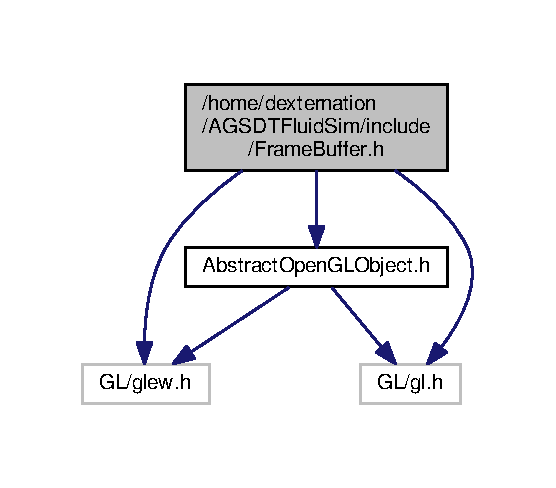
\includegraphics[width=267pt]{_frame_buffer_8h__incl}
\end{center}
\end{figure}
This graph shows which files directly or indirectly include this file\-:\nopagebreak
\begin{figure}[H]
\begin{center}
\leavevmode
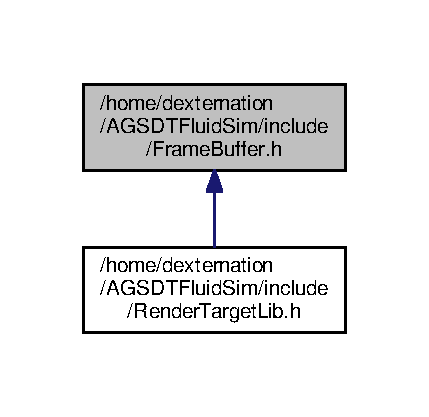
\includegraphics[width=206pt]{_frame_buffer_8h__dep__incl}
\end{center}
\end{figure}
\subsection*{Classes}
\begin{DoxyCompactItemize}
\item 
class \hyperlink{class_frame_buffer}{Frame\-Buffer}
\begin{DoxyCompactList}\small\item\em Class for creating frame buffers. \end{DoxyCompactList}\end{DoxyCompactItemize}

\hypertarget{_g_l_texture_8h}{\section{/home/dexternation/\-A\-G\-S\-D\-T\-Fluid\-Sim/include/\-G\-L\-Texture.h File Reference}
\label{_g_l_texture_8h}\index{/home/dexternation/\-A\-G\-S\-D\-T\-Fluid\-Sim/include/\-G\-L\-Texture.\-h@{/home/dexternation/\-A\-G\-S\-D\-T\-Fluid\-Sim/include/\-G\-L\-Texture.\-h}}
}
{\ttfamily \#include $<$G\-L/glew.\-h$>$}\\*
{\ttfamily \#include $<$G\-L/gl.\-h$>$}\\*
{\ttfamily \#include \char`\"{}Abstract\-Open\-G\-L\-Object.\-h\char`\"{}}\\*
Include dependency graph for G\-L\-Texture.\-h\-:\nopagebreak
\begin{figure}[H]
\begin{center}
\leavevmode
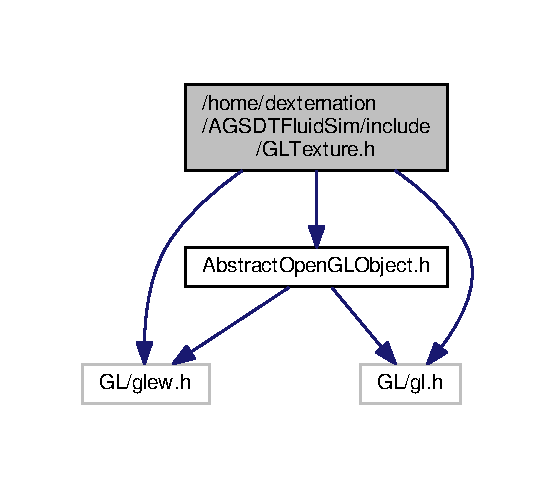
\includegraphics[width=267pt]{_g_l_texture_8h__incl}
\end{center}
\end{figure}
This graph shows which files directly or indirectly include this file\-:\nopagebreak
\begin{figure}[H]
\begin{center}
\leavevmode
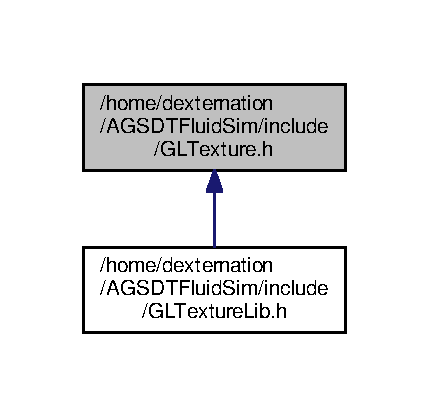
\includegraphics[width=206pt]{_g_l_texture_8h__dep__incl}
\end{center}
\end{figure}
\subsection*{Classes}
\begin{DoxyCompactItemize}
\item 
class \hyperlink{class_g_l_texture}{G\-L\-Texture}
\end{DoxyCompactItemize}

\hypertarget{_g_l_texture_lib_8h}{\section{include/\-G\-L\-Texture\-Lib.h File Reference}
\label{_g_l_texture_lib_8h}\index{include/\-G\-L\-Texture\-Lib.\-h@{include/\-G\-L\-Texture\-Lib.\-h}}
}
{\ttfamily \#include $<$map$>$}\\*
{\ttfamily \#include $<$G\-L\-Texture.\-h$>$}\\*
{\ttfamily \#include $<$string$>$}\\*
Include dependency graph for G\-L\-Texture\-Lib.\-h\-:
\subsection*{Classes}
\begin{DoxyCompactItemize}
\item 
class \hyperlink{class_g_l_texture_lib}{G\-L\-Texture\-Lib}
\begin{DoxyCompactList}\small\item\em Simple class for loading in and managing Open\-G\-L textures. \end{DoxyCompactList}\end{DoxyCompactItemize}

\hypertarget{_open_g_l_widget_8h}{\section{/home/dexternation/\-A\-G\-S\-D\-T\-Fluid\-Sim/include/\-Open\-G\-L\-Widget.h File Reference}
\label{_open_g_l_widget_8h}\index{/home/dexternation/\-A\-G\-S\-D\-T\-Fluid\-Sim/include/\-Open\-G\-L\-Widget.\-h@{/home/dexternation/\-A\-G\-S\-D\-T\-Fluid\-Sim/include/\-Open\-G\-L\-Widget.\-h}}
}
{\ttfamily \#include $<$ngl/\-N\-G\-L\-Init.\-h$>$}\\*
{\ttfamily \#include $<$ngl/\-Mat4.\-h$>$}\\*
{\ttfamily \#include $<$ngl/\-Vec3.\-h$>$}\\*
{\ttfamily \#include $<$ngl/\-Camera.\-h$>$}\\*
{\ttfamily \#include $<$ngl/\-Text.\-h$>$}\\*
{\ttfamily \#include $<$Q\-G\-L\-Widget$>$}\\*
{\ttfamily \#include $<$Q\-Event$>$}\\*
{\ttfamily \#include $<$Q\-Resize\-Event$>$}\\*
{\ttfamily \#include $<$Q\-Message\-Box$>$}\\*
{\ttfamily \#include $<$Q\-String$>$}\\*
{\ttfamily \#include $<$Q\-Time$>$}\\*
{\ttfamily \#include $<$Q\-Color$>$}\\*
{\ttfamily \#include \char`\"{}S\-P\-H\-Engine.\-h\char`\"{}}\\*
{\ttfamily \#include \char`\"{}Fluid\-Shader.\-h\char`\"{}}\\*
Include dependency graph for Open\-G\-L\-Widget.\-h\-:\nopagebreak
\begin{figure}[H]
\begin{center}
\leavevmode
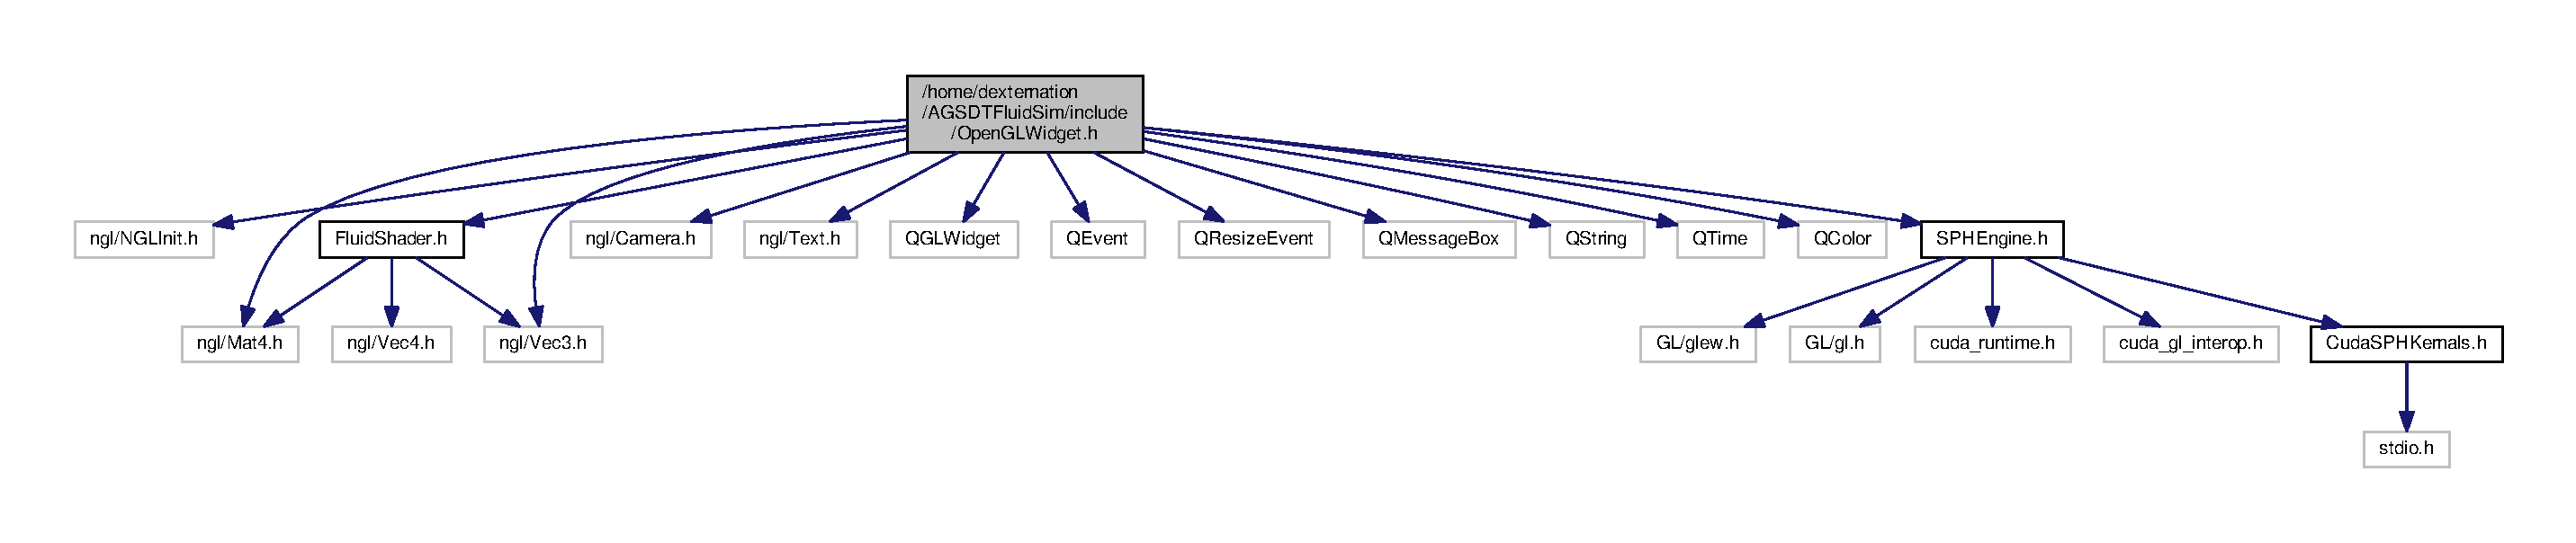
\includegraphics[width=350pt]{_open_g_l_widget_8h__incl}
\end{center}
\end{figure}
This graph shows which files directly or indirectly include this file\-:\nopagebreak
\begin{figure}[H]
\begin{center}
\leavevmode
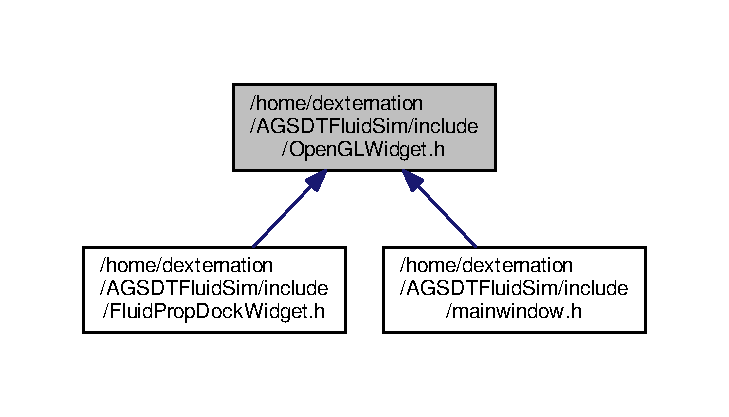
\includegraphics[width=350pt]{_open_g_l_widget_8h__dep__incl}
\end{center}
\end{figure}
\subsection*{Classes}
\begin{DoxyCompactItemize}
\item 
class \hyperlink{class_open_g_l_widget}{Open\-G\-L\-Widget}
\begin{DoxyCompactList}\small\item\em Basic Qt widget that holds a Open\-G\-L context. \end{DoxyCompactList}\item 
struct \hyperlink{struct_open_g_l_widget_1_1fluid_sim_props}{Open\-G\-L\-Widget\-::fluid\-Sim\-Props}
\begin{DoxyCompactList}\small\item\em structure to hold some update information about our fluid simulations \end{DoxyCompactList}\end{DoxyCompactItemize}

\hypertarget{_render_buffer_8h}{\section{include/\-Render\-Buffer.h File Reference}
\label{_render_buffer_8h}\index{include/\-Render\-Buffer.\-h@{include/\-Render\-Buffer.\-h}}
}
{\ttfamily \#include $<$G\-L/glew.\-h$>$}\\*
{\ttfamily \#include $<$G\-L/gl.\-h$>$}\\*
{\ttfamily \#include \char`\"{}Abstract\-Open\-G\-L\-Object.\-h\char`\"{}}\\*
Include dependency graph for Render\-Buffer.\-h\-:
This graph shows which files directly or indirectly include this file\-:
\subsection*{Classes}
\begin{DoxyCompactItemize}
\item 
class \hyperlink{class_render_buffer}{Render\-Buffer}
\begin{DoxyCompactList}\small\item\em Class for creating render buffers. \end{DoxyCompactList}\end{DoxyCompactItemize}

\hypertarget{_render_target_lib_8h}{\section{include/\-Render\-Target\-Lib.h File Reference}
\label{_render_target_lib_8h}\index{include/\-Render\-Target\-Lib.\-h@{include/\-Render\-Target\-Lib.\-h}}
}
{\ttfamily \#include $<$map$>$}\\*
{\ttfamily \#include $<$string$>$}\\*
{\ttfamily \#include \char`\"{}Frame\-Buffer.\-h\char`\"{}}\\*
{\ttfamily \#include \char`\"{}Render\-Buffer.\-h\char`\"{}}\\*
Include dependency graph for Render\-Target\-Lib.\-h\-:
\subsection*{Classes}
\begin{DoxyCompactItemize}
\item 
class \hyperlink{class_render_target_lib}{Render\-Target\-Lib}
\begin{DoxyCompactList}\small\item\em Singleton class for creating and storing render targets in a library. \end{DoxyCompactList}\end{DoxyCompactItemize}

\input{_text_8h}
%--- End generated contents ---

% Index
\newpage
\phantomsection
\addcontentsline{toc}{chapter}{Index}
\printindex

\end{document}
